\documentclass[letterpaper]{article}
\usepackage[plots]{settings}

\begin{document}
\begin{notes}{Part 2: Restoration and Transforms}


\NoteChapter{Noise Models}

Every measured image is a corrupted version of the scene. \textbf{Noise} is the random part of that corruption - the part that changes from one exposure to the next, or that is frozen into the sensor itself. Modelling it matters because every denoiser in the next chapter is optimal only under an assumed noise model, and choosing the wrong one is the usual reason a denoiser disappoints.

\textbf{Observation models.} Three forms cover almost everything:
$$\underbrace{g = f + \eta}_{\text{additive}},\qquad \underbrace{g = f\cdot\eta}_{\text{multiplicative}},\qquad \underbrace{g \sim \mathcal{P}(f)}_{\text{signal-dependent}}.$$

\textbf{Three axes of classification.} Any real noise source is placed by answering three questions:
\begin{enumerate}
    \item \textbf{Additive or multiplicative?} Additive noise is independent of the signal (read noise); multiplicative noise scales with it (speckle, PRNU).
    \item \textbf{Signal-independent or signal-dependent?} Read noise is constant; photon shot noise grows as $\sqrt{S}$.
    \item \textbf{Temporal or fixed-pattern?} This is the practically decisive one. \emph{Temporal} noise is redrawn every frame, so averaging $N$ frames reduces it by $\sqrt{N}$. \emph{Fixed-pattern} noise (FPN) is the same in every frame, so it \textbf{does not average away} - it must be measured and calibrated out.
\end{enumerate}

\begin{figure}[H]
    \centering
    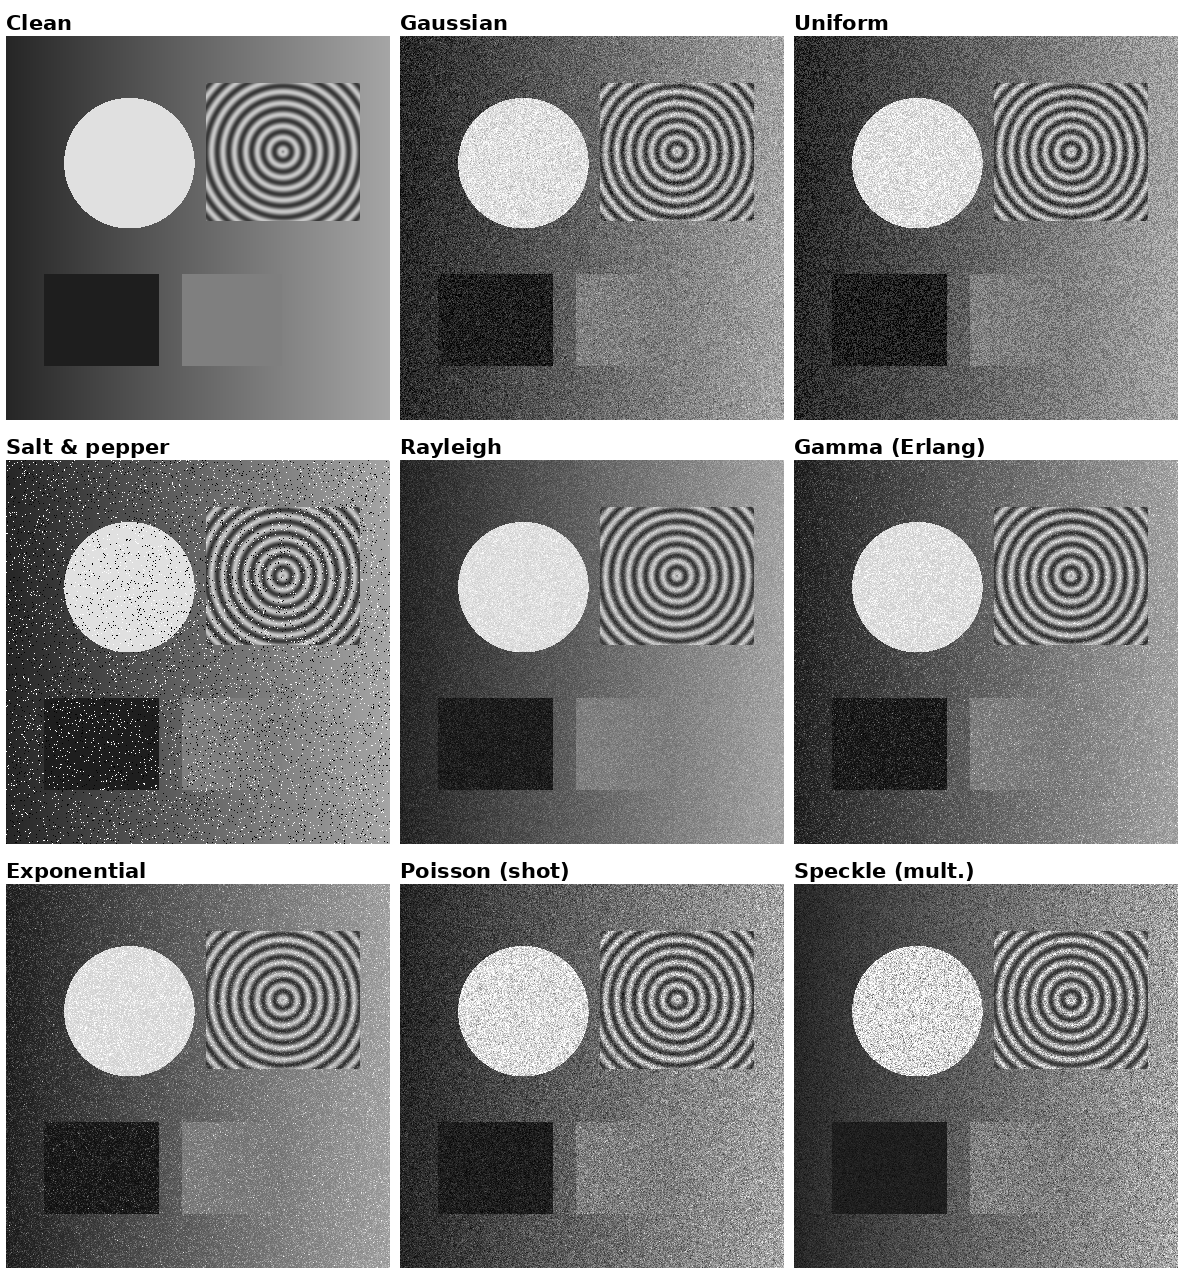
\includegraphics[width=1\linewidth]{images/part2/noise-gallery.png}
    \caption{The same synthetic scene under each noise model. Note that Poisson and speckle noise are visibly stronger on the bright disk than on the dark square - their severity tracks the signal - whereas Gaussian and uniform noise are uniform across the frame.}
\end{figure}

\NoteSection{Why Noise Exists}

Noise is not a manufacturing defect waiting to be engineered away. It has four independent physical roots, and only the last two are even partly under a designer's control.

\textbf{1. Light is quantised.} A source emits photons as discrete, mutually independent events, so the number $N$ arriving at a pixel during an exposure is a Poisson random variable with
$$\mathrm{Var}[N] = \mathrm{E}[N] = \lambda.$$
Note that nothing about the detector appears in that statement - the randomness is in the light \emph{before it arrives}. A hypothetical perfect camera (quantum efficiency $1$, zero dark current, zero read noise, infinite bit depth) pointed at a perfectly static scene would still record a different number at every pixel on every exposure.

\textbf{2. Temperature is not zero.} Any component at $T>0$ carries thermal energy on the order of $kT$ per degree of freedom, which leaks into the measurement three ways:
\begin{itemize}
    \item carriers are thermally excited across the silicon bandgap, giving \emph{dark current} $\propto e^{-E_g/2kT}$;
    \item any resistance generates \emph{Johnson-Nyquist} noise, $\overline{v_n^2} = 4kTR\,\Delta f$;
    \item resetting the sense capacitor $C$ leaves a random charge, \emph{$kTC$ noise}, of $\sigma_Q=\sqrt{kTC}$ coulombs.
\end{itemize}
Cooling suppresses all three, which is exactly why scientific cameras are cooled - but $T=0$ is unattainable.

\textbf{3. Charge is discrete, and measurement must be amplified.} A current is a countable stream of electrons, so it necessarily fluctuates (Schottky shot noise, $\overline{i_n^2}=2qI\,\Delta f$). Reading the signal out requires amplification, and every amplifier adds noise of its own - no amplifier improves SNR, it can only degrade it less or more.

\textbf{4. Fabrication is imperfect.} Doping density, oxide thickness, microlens alignment and pixel geometry all vary at the scale of the individual pixel, so no two pixels share exactly the same gain and offset. This variation is \emph{deterministic} - frozen in at manufacture - but unknown, so it behaves as noise until it is measured. This is the fixed-pattern noise of the later sections.

\textbf{The fundamental limit.} Sources 2-4 can be reduced by cooling, better circuits and calibration. Source 1 cannot be reduced at all. Since $\sigma=\sqrt\lambda$ for Poisson statistics,
$$\mathrm{SNR} = \frac{\lambda}{\sqrt{\lambda}} = \sqrt{\lambda},$$
so \textbf{doubling the SNR requires four times the photons}. This is a statement about physics, not about engineering, and it is the reason low-light imaging is fundamentally hard: the only remedies are a longer exposure, a wider aperture, or larger pixels - all of which simply collect more photons.

\begin{figure}[H]
    \centering
    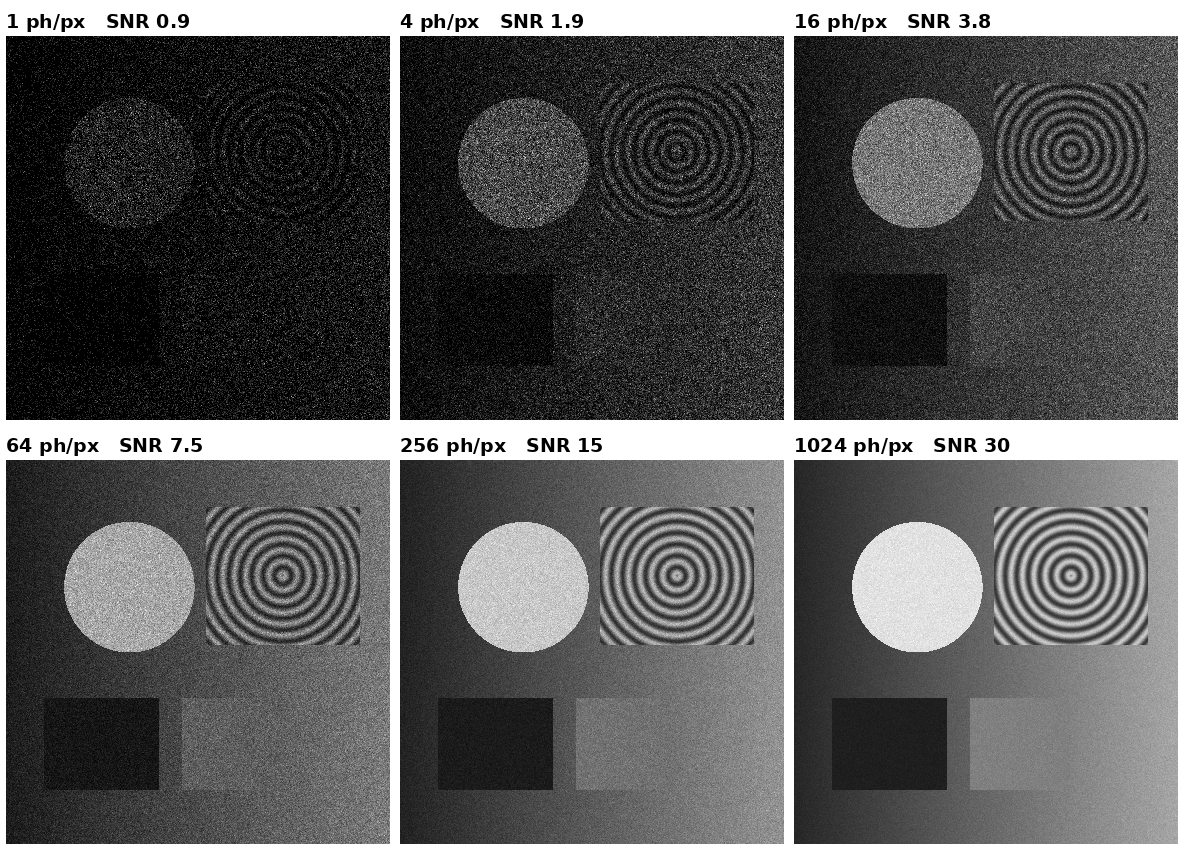
\includegraphics[width=1\linewidth]{images/part2/photon-limit.png}
    \caption{The same scene recorded by an \emph{ideal, noiseless} detector as the photon budget grows. Every trace of grain here is the arrival statistics of the light itself; no sensor imperfection is modelled. The scene emerges only as $\sqrt\lambda$ grows, illustrating why more light - and nothing else - is the cure for shot noise.}
\end{figure}

\textbf{Why not simply average it away?} Temporal noise does fall as $1/\sqrt N$ over $N$ frames, but averaging costs time: the scene or camera must hold still, or the gain in SNR is paid for in motion blur. And fixed-pattern noise, being identical in every frame, does not average down at all - averaging converges to the pattern rather than removing it.

\textbf{Noise versus distortion.} Blur, vignetting and lens aberration are \emph{deterministic} degradations - identical every exposure, and therefore invertible in principle, which is the subject of the DEBLURRING chapter. Noise is random and irreversible: no filter recovers the value that was actually lost, it can only estimate it. This is precisely why deconvolution and denoising are treated as separate problems, and why the two are in tension - sharpening amplifies noise, and smoothing destroys detail.

\NoteSection{The Imaging Chain: Where Noise Enters}

A photon becomes a number through a fixed sequence of stages, and each contributes its own noise:
\begin{enumerate}
    \item \textbf{Photon arrival.} Inherently random (Poisson) - shot noise, present before the sensor does anything.
    \item \textbf{Photoelectric conversion.} Quantum efficiency $\eta$ (electrons per incident photon) sets how many photons are captured at all.
    \item \textbf{Charge integration.} Thermally generated electrons accumulate alongside signal electrons - dark current.
    \item \textbf{Readout.} The source-follower amplifier adds read noise; the reset transistor adds $kTC$ noise.
    \item \textbf{Bias offset.} A deliberate electronic pedestal $B$ keeps the ADC from clipping negative noise excursions.
    \item \textbf{Quantisation.} The ADC rounds to discrete digital numbers (DN), adding uniform noise.
\end{enumerate}

Collecting these, the digital value at a pixel is
$$I = G\bigl(\underbrace{\eta\,\Phi\,t}_{\text{photoelectrons}} + \underbrace{D(T)\,t}_{\text{dark}}\bigr) + \underbrace{B}_{\text{bias}} + \eta_{\text{read}} + \eta_{\text{quant}},$$
where $G$ is the gain in DN per electron, $\Phi$ the photon flux, $t$ the exposure time, and $D(T)$ the dark-current rate in electrons per pixel per second. Every term on the right is a separate noise source, and the rest of this chapter takes them one at a time.

\NoteSection{Gaussian Noise}

Models electronic and thermal noise:
$$p(z) = \frac{1}{\sqrt{2\pi}\,\sigma}\exp\!\left(-\frac{(z-\mu)^2}{2\sigma^2}\right), \quad \text{mean } \mu,\ \text{variance } \sigma^2.$$

\textbf{Why it dominates.} By the central limit theorem, any sum of many small independent perturbations tends to Gaussian regardless of the individual distributions. Read noise is the sum of many such contributions, so it is Gaussian to excellent accuracy.

\textbf{AWGN.} The standard assumption is \emph{additive white Gaussian noise}: samples are independent across pixels (white, so a flat power spectrum) and independent of $f$. Then $\Sigma_\eta=\sigma^2 I$.

\textbf{Consequences.} Tractable: linear filters (Wiener, mean) are MSE-optimal under Gaussian assumptions, and the maximum-likelihood estimate is a least-squares fit. This is why so much restoration theory silently assumes it.

\NoteSection{Uniform and Quantisation Noise}

All intensities in $[a,b]$ equally likely:
$$p(z)=\tfrac{1}{b-a},\quad a\le z\le b; \qquad \mu=\tfrac{a+b}{2},\quad \sigma^2=\tfrac{(b-a)^2}{12}.$$

\textbf{Quantisation.} The standard physical instance. An ADC with step size $q$ rounds each value, giving an error uniform on $[-q/2, q/2]$ and hence
$$\sigma_q^2 = \frac{q^2}{12}.$$
For an $n$-bit converter over full scale $F$, $q = F/2^n$, so each extra bit halves the quantisation noise.

\textbf{When it matters.} Quantisation should sit \emph{below} the read noise floor. If read noise is much smaller than $q$ the image is quantisation-limited and shows visible banding in smooth gradients. The fix is \emph{dithering}: adding a small amount of noise before quantising decorrelates the error from the signal, trading banding for a slightly higher but far less visible noise floor.

\NoteSection{Impulse (Salt-and-Pepper) Noise}

Random pixels snapped to maximum (salt, white) or minimum (pepper, black):
$$p(z) = \begin{cases}P_a, & z=0\ (\text{pepper}),\\ P_b, & z=L{-}1\ (\text{salt}),\\ 1{-}P_a{-}P_b, & \text{otherwise.}\end{cases}$$

\textbf{Causes.} Dead or stuck pixels in the sensor array, bit errors in transmission or storage, and analogue-to-digital converter faults. Unlike the other models here it is not a perturbation of the true value - the original value is \emph{destroyed}.

\textbf{Consequences.} Because the corrupted values are \emph{outliers} rather than perturbations, no linear filter can help - averaging merely spreads the spike over the neighbourhood, replacing one bad pixel with nine mediocre ones. Impulse noise is the one case where order statistics beat every linear method outright (see DENOISING, order-statistic filters).

\NoteSection{Rayleigh Noise}

Skewed right; arises in range and sonar imaging:
$$p(z)=\tfrac{2(z-a)}{b}e^{-(z-a)^2/b},\;\;z\ge a;\quad \mu=a+\sqrt{\pi b/4},\;\;\sigma^2=b(4{-}\pi)/4.$$

\textbf{Where it comes from.} The Rayleigh distribution is the magnitude of a complex number whose real and imaginary parts are independent zero-mean Gaussians. Any imaging method that measures the \emph{envelope} of a complex signal therefore produces Rayleigh-distributed noise in dark regions - magnitude MRI, radar and sonar returns, and ultrasound envelopes. Its non-zero mean is why MRI background regions look grey rather than black.

\textbf{Consequences.} Because the noise is the magnitude of a complex quantity, its effect is a signal-dependent \emph{bias} rather than signal-dependent variance - the general case is the Rician distribution, of which Rayleigh is the zero-signal limit. Removing the bias before denoising is what the treatment in DENOISING addresses.

\NoteSection{Gamma (Erlang) Noise}

Models laser speckle:
$$p(z)=\frac{a^b z^{b-1}}{(b-1)!}e^{-az},\;\;z\ge 0;\quad \mu=b/a,\;\;\sigma^2=b/a^2.$$

\textbf{Interpretation.} The sum of $b$ independent exponential variables. In coherent imaging the parameter $b$ counts \emph{looks}: averaging $b$ independent speckle realisations of the same scene turns exponential statistics into Gamma statistics with $b$ degrees of freedom. The exponent $b$ is therefore a direct measure of how much speckle has already been suppressed at acquisition time (see DENOISING, multi-look averaging).

\NoteSection{Exponential Noise}

Special case of Gamma ($b=1$):
$$p(z) = a\,e^{-az},\;\;z\ge 0;\quad \mu=1/a,\;\;\sigma^2=1/a^2.$$
Arises in laser and ultrasound imaging. Note $\sigma = \mu$: single-look coherent intensity imagery has 100\% relative noise, which is why raw SAR looks so grainy.

\NoteSection{Poisson (Photon Shot) Noise}

Dominant in photon-limited imaging (astronomy, fluorescence microscopy, low-dose CT). For a pixel collecting a mean of $\lambda$ photons:
$$P(z=k)=\frac{e^{-\lambda}\lambda^k}{k!},\qquad \sigma^2 = \lambda,\qquad \mathrm{SNR}=\frac{\lambda}{\sqrt\lambda}=\sqrt{\lambda}.$$

\textbf{Irreducible.} This is not a defect of the sensor - it is the quantum statistics of light itself. A perfect noiseless detector still measures Poisson-distributed counts. The only way to improve SNR is to collect more photons (longer exposure, wider aperture, larger pixels).

\textbf{Consequences.} At high flux Poisson$\to$Gaussian with $\sigma^2=\lambda$, so a Gaussian denoiser is adequate once the signal level is known. At low flux the variance changes from pixel to pixel with the signal itself, and the standard remedy is to stabilise it first (see DENOISING, variance stabilisation).

\NoteSection{Speckle (Multiplicative) Noise}

In \emph{coherent} imaging - SAR, ultrasound, OCT, laser illumination - many sub-resolution scatterers within one resolution cell return waves that interfere. The result is multiplicative:
$$g(x,y) = f(x,y)\cdot\eta(x,y),\qquad \mathrm{E}[\eta]=1.$$

\textbf{Why it is not really ``noise''.} Speckle is deterministic given the exact scatterer positions - re-imaging the identical scene reproduces it. It is treated statistically only because the microstructure is unknowable.

\textbf{Statistics.} For fully developed speckle the intensity is exponentially distributed, so $\sigma=\mu$ - a relative noise level of $100\%$ in single-look data, independent of how bright the scene is. Averaging independent looks is the only way to reduce it at acquisition; afterwards, the multiplicative structure must be converted to additive form before any standard denoiser applies (see DENOISING, variance stabilisation).

\NoteSection{Bias (Offset) and Read Noise}

\textbf{Bias (offset).} A deliberate constant pedestal $B$ added before the ADC so that negative noise excursions around zero signal are not clipped. It is a \emph{deterministic, reproducible} quantity, not noise - which means it can be measured once and subtracted exactly. It is not perfectly flat: readout electronics impose faint column- and row-wise structure on it.

\textbf{Read noise.} The genuinely random part of readout, contributed by the source-follower amplifier and the ADC. Quoted in electrons RMS ($\sigma_r$), typically $1$-$10\,e^-$ for modern CMOS and under $1\,e^-$ for scientific sensors. Crucially it is \textbf{independent of both exposure time and signal level}, so it sets the noise floor of the sensor.

\textbf{Components.}
\begin{itemize}
    \item \textbf{Reset ($kTC$) noise.} Resetting the sense node leaves an uncertain charge with $\sigma = \sqrt{kTC}/q$ electrons. Removed by \emph{correlated double sampling} (CDS): sample the node right after reset and again after integration, and subtract - the common reset level cancels.
    \item \textbf{$1/f$ flicker noise.} Low-frequency amplifier drift; also suppressed by CDS.
    \item \textbf{ADC noise.} Quantisation plus converter non-idealities.
\end{itemize}

\textbf{Why it matters.} Read noise fixes the \emph{dynamic range} of the sensor,
$$\mathrm{DR} = \frac{\text{full-well capacity}}{\sigma_r},\qquad \mathrm{DR_{dB}} = 20\log_{10}\frac{\text{FW}}{\sigma_r},$$
and it dominates the total noise in every dark or short-exposure image.

\NoteSection{Dark Current and Thermal Noise}

\textbf{Dark current.} Thermal energy alone frees electrons in the silicon depletion region, and the pixel cannot distinguish them from photoelectrons. The accumulated \emph{dark signal} is
$$S_{\text{dark}} = D(T)\cdot t \quad [e^-],$$
proportional to exposure time and strongly dependent on temperature:
$$D(T) \propto T^{3/2}\,e^{-E_g/2kT} \;\;\Longrightarrow\;\; D(T) \approx D(T_0)\cdot 2^{(T-T_0)/\Delta T},\quad \Delta T\approx 6\text{-}7^\circ\mathrm{C}.$$
As a rule of thumb, \textbf{dark current doubles for every $6$-$7^\circ$C rise}. This is the entire reason scientific and astronomical cameras are cooled, often to $-70^\circ$C, where dark current becomes negligible even over hour-long exposures.

\textbf{The critical distinction.} The dark \emph{signal} $Dt$ is deterministic and can be subtracted exactly. The dark \emph{shot noise} $\sqrt{Dt}$ is Poisson and \textbf{cannot} - subtracting a dark frame removes the mean but leaves (in fact slightly increases) the random part. Cooling is the only way to reduce it.

\textbf{Hot pixels.} Individual pixels with crystal defects have dark current orders of magnitude above the array median. They appear as isolated bright dots that grow with exposure time and temperature, and are usually handled by a defect map plus interpolation rather than by subtraction.

\textbf{Amplifier glow.} Infrared emission from on-chip readout electronics exposes the nearby corner of the array, producing a characteristic glow in long exposures (visible in the dark frame in the next figure).

\NoteSection{Fixed-Pattern Noise: DSNU and PRNU}

Fixed-pattern noise is spatial non-uniformity that repeats identically in every frame. It splits into an offset term and a gain term:

\begin{itemize}
    \item \textbf{DSNU} (dark signal non-uniformity) - pixel-to-pixel variation in \emph{dark current}. Additive, independent of illumination, grows with exposure time. Removed by \textbf{dark-frame subtraction}.
    \item \textbf{PRNU} (photo-response non-uniformity) - pixel-to-pixel variation in \emph{gain}, from variations in pixel area, microlens alignment and quantum efficiency. Multiplicative, typically $0.5$-$2\%$ of signal. Removed by \textbf{flat-field division}.
\end{itemize}

Writing both into the model, a pixel responds as
$$I_{ij} = K_{ij}\,S_{ij} + O_{ij} + \eta,$$
with gain map $K$ (PRNU) and offset map $O$ (DSNU + bias).

\textbf{Why PRNU sets the ceiling.} Because PRNU noise is $p\cdot S$ with $p$ constant, it grows \emph{linearly} with signal while shot noise grows only as $\sqrt S$. At high signal levels PRNU therefore overtakes everything else and the SNR stops improving, saturating at $1/p$ - roughly $50$-$200{:}1$. Flat fielding is what removes this ceiling.

\NoteSection{Row, Column, and Random Telegraph Noise}

Not all noise is spatially independent, and the eye is far more sensitive to structure than to grain.

\textbf{Column FPN.} CMOS sensors use one amplifier and often one ADC per column, so each column carries a slightly different offset. The result is vertical banding, clearly visible in the master bias frame in the next figure.

\textbf{Row noise.} Shared readout circuitry and supply fluctuations vary between rows, giving horizontal streaks that change frame to frame. Commonly corrected using \emph{optical black} pixels - a masked region at the edge of the array that sees no light, whose per-row mean estimates the offset to subtract.

\textbf{Random telegraph signal (RTS).} In very small pixels a single trap capturing and releasing a charge carrier makes the pixel switch discretely between two or more output levels. The result is ``blinking'' pixels that cannot be removed by a static defect map because the level changes randomly in time.

\textbf{Practical note.} Because banding is structured, it is objectionable at amplitudes far below what would be acceptable for white noise. Sensor vendors spend disproportionate effort on it for this reason.

\NoteSection{The Total Noise Budget and SNR}

Independent noise sources add in \emph{variance}. In electrons, for a signal of $S$ electrons:
$$\sigma_{\text{tot}}^2 = \underbrace{S}_{\text{photon shot}} + \underbrace{D t}_{\text{dark shot}} + \underbrace{\sigma_r^2}_{\text{read}} + \underbrace{(pS)^2}_{\text{PRNU}} + \underbrace{\sigma_q^2}_{\text{quant}},$$
giving
$$\mathrm{SNR} = \frac{S}{\sqrt{S + Dt + \sigma_r^2 + (pS)^2}}.$$

\textbf{Three regimes.} Which term dominates depends entirely on signal level:
\begin{enumerate}
    \item \textbf{Read-noise limited} ($S \ll \sigma_r^2$): $\mathrm{SNR}\approx S/\sigma_r$, growing \emph{linearly} with signal. Dark scenes, short exposures, high frame rates.
    \item \textbf{Shot-noise limited} (mid range): $\mathrm{SNR}\approx\sqrt S$. The desirable regime - performance is set by physics, not by the sensor.
    \item \textbf{PRNU limited} ($pS \gg \sqrt S$): $\mathrm{SNR}\to 1/p$, flat. No further gain from more light; only flat fielding helps.
\end{enumerate}

\begin{center}
\begin{tikzpicture}
\begin{axis}[notesplot, xmode=log, ymode=log,
    xlabel={signal $S$ (e$^-$)}, ylabel={noise $\sigma$ (e$^-$)},
    legend pos=north west, legend cell align=left]
\addplot[domain=0:5, samples=140] ({10^x},{sqrt(25 + 10^x + (0.01*10^x)^2)});
\addlegendentry{total}
\addplot[dashed, domain=0:5, samples=2] ({10^x},{5});
\addlegendentry{read floor ($\sigma_r$)}
\addplot[dotted, domain=0:5, samples=140] ({10^x},{sqrt(10^x)});
\addlegendentry{shot ($\sqrt S$)}
\addplot[dashdotted, domain=0:5, samples=140] ({10^x},{0.01*10^x});
\addlegendentry{PRNU ($pS$)}
\end{axis}
\end{tikzpicture}
\end{center}

\NoteSection{Sensor Calibration: Bias, Dark and Flat Frames}

The deterministic parts of the model - bias, dark signal and PRNU - are measured with three calibration frames and removed arithmetically.

\begin{enumerate}
    \item \textbf{Bias frame.} Zero-length exposure with the shutter closed. Captures the offset pedestal $B$ and its column structure.
    \item \textbf{Dark frame.} Shutter closed, \emph{same exposure time and temperature} as the real image. Captures $B + Dt$, including hot pixels and amp glow.
    \item \textbf{Flat field.} Uniformly illuminated scene. Captures the multiplicative gain map: PRNU, lens vignetting and dust shadows together.
\end{enumerate}

\textbf{Master frames.} Each is the average of many individual frames. Averaging $N$ frames divides the \emph{temporal} noise by $\sqrt N$, leaving an essentially noise-free estimate of the fixed pattern - otherwise calibration would inject as much noise as it removes.

\textbf{The correction.} With master frames $\mathcal{B}$, $\mathcal{D}$, $\mathcal{F}$, the calibrated image is
$$\hat f = \frac{g - \mathcal{D}}{\mathcal{F} - \mathcal{B}}\cdot\bigl\langle \mathcal{F} - \mathcal{B}\bigr\rangle,$$
where $\langle\cdot\rangle$ denotes the spatial mean, included to preserve the overall intensity scale. Note $\mathcal{D}$ already contains the bias, so subtracting it removes both at once.

\begin{figure}[H]
    \centering
    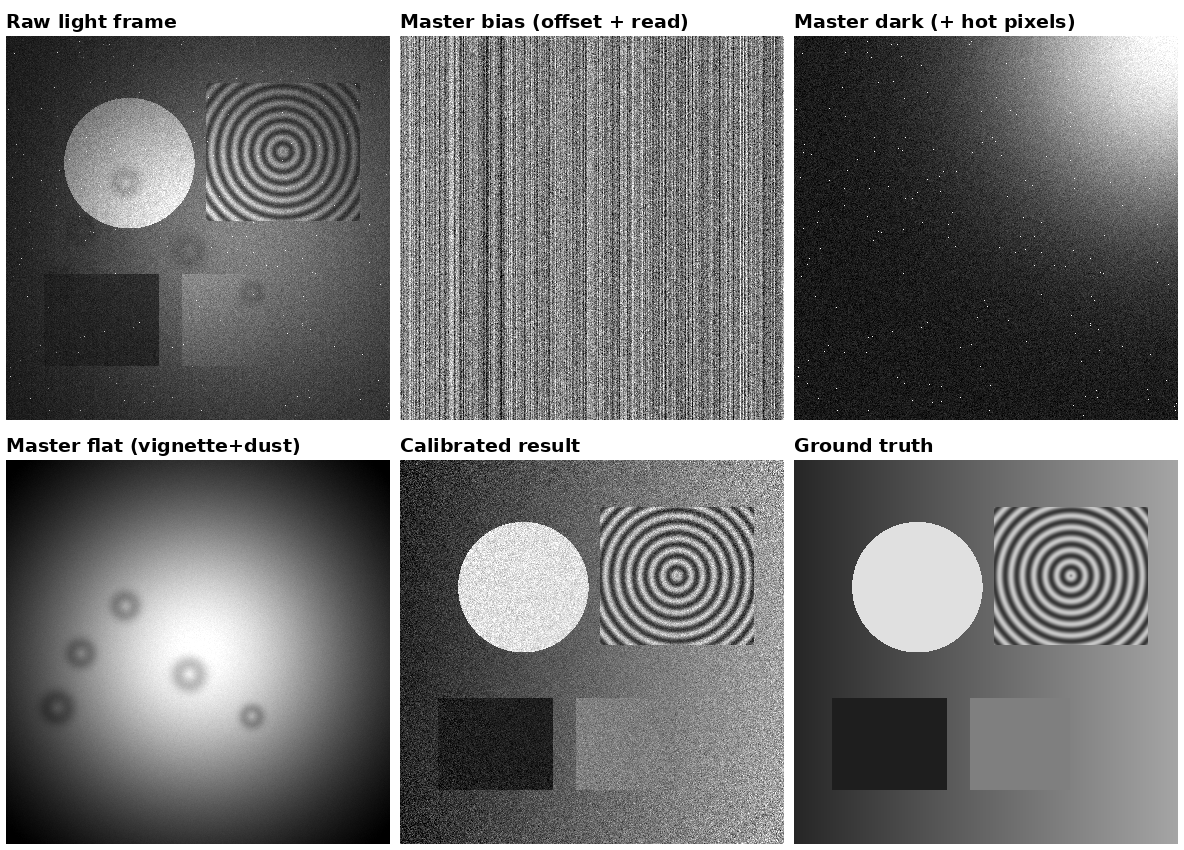
\includegraphics[width=1\linewidth]{images/part2/sensor-calibration.png}
    \caption{The calibration pipeline. The bias and dark frames are contrast-stretched to make their structure visible. Column banding is apparent in the bias; amplifier glow and hot pixels in the dark; vignetting and dust motes in the flat. Subtracting the dark and dividing by the flat recovers the scene, though the shot and read noise - the genuinely random parts - necessarily remain.}
\end{figure}

\textbf{What calibration cannot do.} It removes only the deterministic terms. Shot noise, dark shot noise and read noise survive untouched, and subtracting a noisy dark frame actually \emph{adds} its noise in quadrature - hence the insistence on averaged masters.

\NoteSection{The Photon Transfer Curve}

The \textbf{photon transfer curve} (PTC) is the standard experimental method for characterising a sensor, and it recovers the parameters above without opening the camera. Capture pairs of flat-field frames at increasing illumination; for each pair plot the noise $\sigma$ against the mean signal $S$, both in DN, on log-log axes. Differencing the two frames of a pair cancels the fixed pattern, isolating temporal noise.

The curve shows the three regimes as three straight lines:
\begin{itemize}
    \item slope $0$ - the read-noise floor, whose height gives $\sigma_r$;
    \item slope $1/2$ - the shot-noise region. Since $\sigma_{DN}^2 = S_{DN}/K$ for conversion gain $K$ in $e^-$/DN, fitting this region measures $K$ - the only practical way to convert DN to electrons;
    \item slope $1$ - the PRNU region (present only if the fixed pattern has not been differenced away), whose height gives $p$.
\end{itemize}
The signal at which the curve turns over and collapses marks the \textbf{full-well capacity}. Together with $\sigma_r$ this yields the dynamic range.

\NoteSection{Noise in the Colour Pipeline}

Everything above describes a single monochrome measurement. A colour camera then applies a processing chain, and each stage reshapes the noise:

\begin{enumerate}
    \item \textbf{Colour filter array.} Each pixel measures one of R, G, B, so each channel is sampled at a fraction of the full resolution, and each filter discards roughly two-thirds of the incoming light - an immediate SNR cost.
    \item \textbf{Demosaicing.} Interpolating the missing channels makes neighbouring pixels linear combinations of shared measurements. Noise that was independent per pixel becomes \emph{spatially correlated} and correlated \emph{between channels} - which is why post-demosaic denoising is much harder, and why raw-domain denoising is preferred.
    \item \textbf{White balance.} Channels are multiplied by different gains. Under tungsten light the blue gain may exceed $2\times$, amplifying blue-channel noise correspondingly; the noisiest channel is usually the one least matched to the illuminant.
    \item \textbf{Colour matrix.} Mixing channels to reach the output colour space further correlates their noise, typically amplifying \emph{chroma} noise.
    \item \textbf{Gamma / tone curve.} A concave curve steeply amplifies shadows, so noise that was uniform in linear space becomes strongly signal-dependent in the output - loudest exactly where the signal is weakest.
\end{enumerate}

\textbf{Luma versus chroma.} Human vision has far lower spatial acuity for colour than for luminance, so chroma noise appears as large, slow, blotchy patches and is judged more objectionable than fine luma grain. Practical denoisers exploit this by working in a luma-chroma space and filtering the chroma channels far more aggressively.

\NoteSection{Estimating Noise from a Single Image}

Restoration filters need $\sigma_\eta$, but it is rarely supplied. Three standard estimators:

\textbf{Flat-patch variance.} Select a near-uniform (flat) patch of the image; the sample variance in that patch $\approx\sigma_\eta^2$, since true-image variation is negligible there. Simple but requires a human to choose the patch. Automated variant: compute the variance of many small blocks and take a low percentile, on the assumption that the least-varying blocks contain no structure.

\textbf{Robust MAD estimator.} The workhorse. Take the finest-scale diagonal wavelet subband $HH_1$, which contains almost no image structure, and use the median absolute deviation:
$$\hat\sigma_\eta = \frac{\mathrm{median}\bigl(|w_{HH_1}|\bigr)}{0.6745},$$
where $0.6745$ is the MAD of a unit Gaussian. The median makes it insensitive to the few genuine edges that leak into the subband. This is the estimator used for wavelet denoising thresholds later in this part.

\textbf{Laplacian convolution (Immerk\ae r).} Convolve with a kernel designed to annihilate locally linear intensity and respond only to noise:
$$L = \begin{bmatrix}1 & -2 & 1\\ -2 & 4 & -2\\ 1 & -2 & 1\end{bmatrix},\qquad \hat\sigma_\eta = \sqrt{\frac{\pi}{2}}\,\frac{1}{6(W-2)(H-2)}\sum_{x,y}\bigl|(g*L)(x,y)\bigr|.$$
Fast, needs no patch selection, but biased upward on heavily textured images.

\columnbreaknofill

\NoteChapter{Denoising}

Denoising estimates $f$ from a randomly corrupted $g$. It is a different problem from the deblurring of the next chapter, and the distinction is worth stating precisely: blur is a deterministic operator and is invertible in principle, whereas noise destroys information outright. No denoiser recovers the value that was actually measured away - it can only produce a plausible estimate, using a prior about what images look like to decide which of the many signals consistent with $g$ to return.

\textbf{The common structure.} Every method in this chapter separates signal from noise by finding a representation in which the two behave differently, then suppressing whatever looks like noise there:
\begin{itemize}
    \item \textbf{A neighbourhood.} Pixels near each other usually share a value, while their noise is independent - so averaging a neighbourhood cancels noise and preserves signal. Everything hinges on choosing a neighbourhood that does not straddle an edge, which is what separates a mean filter from a bilateral or non-local one.
    \item \textbf{A transform basis.} Natural images are \emph{sparse} in a wavelet or DCT basis - a few large coefficients - while white noise is spread evenly across all of them. Thresholding then removes noise almost exclusively.
    \item \textbf{A frequency.} Periodic interference occupies a few isolated points of the spectrum and nothing else, so it can be excised exactly.
\end{itemize}

\textbf{Know the model first.} Each method is optimal only under an assumed noise model, which is why the previous chapter came first. Most of the machinery below assumes additive white Gaussian noise of known variance, so the chapter opens by reducing the other models to that case, and closes with a table matching noise type to method.

\NoteSection{Variance Stabilisation and Signal-Dependent Noise}

Poisson, speckle, Gamma and Rayleigh noise all break the AWGN assumption in the same way: the noise level is a function of the signal, so a single $\sigma_\eta$ does not exist. All four are handled by the same three-step strategy - \emph{stabilise, denoise, invert}:
\begin{enumerate}
    \item apply a pointwise transform $T$ chosen to make the variance constant;
    \item denoise the transformed image with any AWGN method;
    \item apply $T^{-1}$ to return to intensity units.
\end{enumerate}

\textbf{Choosing $T$.} If the noise standard deviation at signal level $\mu$ is $\sigma(\mu)$, then to first order a pointwise map $T$ propagates it as
$$\mathrm{Var}\bigl[T(z)\bigr] \approx \bigl[T'(\mu)\bigr]^2\sigma^2(\mu),$$
so the variance is constant precisely when $T'(\mu)\propto 1/\sigma(\mu)$, giving the \emph{variance-stabilising transform}
$$T(z) = \int^z \frac{d\mu}{\sigma(\mu)}.$$
The two classical transforms are just this integral evaluated for the two common cases.

\textbf{Anscombe transform (Poisson).} Here $\sigma(\mu)=\sqrt\mu$, so $T(z)\propto\int \mu^{-1/2}d\mu = 2\sqrt{z}$. The standard form adds an offset that improves the approximation at low counts:
$$z\;\longmapsto\;2\sqrt{z+3/8},$$
after which the variance is $\approx 1$ regardless of $\lambda$. The naive inverse $(\,\cdot/2)^2-3/8$ is biased, and at low counts the \emph{exact unbiased inverse} matters more than the choice of denoiser - the bias is a systematic darkening of exactly the faint structure the denoiser was meant to preserve.

\textbf{Homomorphic filtering (multiplicative).} For $g=f\cdot\eta$ the noise scales with the signal, $\sigma(\mu)=c\,\mu$, so $T(z)\propto\int\mu^{-1}d\mu=\log z$ - and indeed
$$\log g = \log f + \log\eta$$
is additive. Denoise the log-image and exponentiate. The catch is that $\mathrm{E}[\log\eta]\ne\log\mathrm{E}[\eta]=0$, so the exponentiated result is biased low by a constant factor that must be restored.

\textbf{Multi-look averaging.} When the acquisition can supply several independent realisations - $b$ \emph{looks} of the same scene in SAR, or repeated frames - averaging them reduces the relative variance by $1/b$ and turns exponential statistics into Gamma statistics with $b$ degrees of freedom. This is the only speckle reduction that adds information rather than trading it away, but it costs spatial resolution (or acquisition time) proportionally.

\textbf{Adaptive coefficient-of-variation filters.} The \textbf{Lee filter} avoids the log entirely, adapting directly to local statistics in the multiplicative model. With local mean $\bar g$ and variance $\sigma_L^2$ over a window, and $C_u$ the known coefficient of variation of the noise,
$$\hat f = \bar g + W\,(g - \bar g),\qquad W = 1 - \frac{C_u^2}{C_g^2},\qquad C_g = \frac{\sigma_L}{\bar g}.$$
In a homogeneous region $C_g\to C_u$, so $W\to0$ and the output is the local mean (full smoothing); across an edge $C_g\gg C_u$, so $W\to1$ and the pixel passes through untouched. This is the multiplicative analogue of the adaptive local noise-reduction filter below, with the coefficient of variation replacing the variance. \textbf{Frost} and \textbf{Kuan} are refinements using the same local-statistics principle.

\textbf{Rayleigh and Rician (envelope) data.} Magnitude images from MRI, radar and ultrasound are the modulus of a complex measurement, so the problem is not heteroscedasticity but \emph{bias}: with underlying amplitude $A$ and per-channel noise $\sigma$,
$$\mathrm{E}\bigl[M^2\bigr] = A^2 + 2\sigma^2,$$
so the squared magnitude is inflated by a constant $2\sigma^2$ - which is why MRI background reads grey rather than black. Correcting to $\hat A = \sqrt{\max(M^2-2\sigma^2,\,0)}$ before applying an ordinary denoiser is the standard fix. Better still, denoise the complex data \emph{before} taking the magnitude, when it is available: the noise there is genuinely additive Gaussian and no correction is needed.

\textbf{When not to stabilise.} At very low photon counts ($\lambda\lesssim1$) no pointwise transform makes the distribution acceptably Gaussian, and stabilise-then-denoise loses to methods that model the Poisson likelihood directly - Richardson--Lucy, or a variational objective with a Poisson data term.

\NoteSection{Spatial Noise Reduction Filters}

Given $g = f + \eta$, a spatial filter estimates $\hat{f}(x,y)$ from the $m\times n$ neighbourhood $S_{xy}$.

\NoteSubsection{Mean Filters}

\textbf{Arithmetic mean.} $\hat{f} = \frac{1}{mn}\sum_{S_{xy}}g(s,t)$. Blurs edges; optimal for Gaussian noise.

\textbf{Geometric mean.} $\hat{f} = \bigl(\prod_{S_{xy}}g(s,t)\bigr)^{1/(mn)}$. Similar smoothing but loses less detail; fails if any pixel is zero.

\textbf{Harmonic mean.} $\hat{f} = mn\!\Big/\!\sum_{S_{xy}}\frac{1}{g(s,t)}$. Handles Gaussian and \emph{salt} noise; fails for pepper noise.

\textbf{Contraharmonic mean (order $Q$).}
$$\hat{f} = \frac{\sum g^{Q+1}}{\sum g^{Q}}.$$
$Q>0$: eliminates pepper noise. $Q<0$: eliminates salt noise. $Q=0$: arithmetic mean; $Q=-1$: harmonic mean.

\NoteSubsection{Order-Statistic Filters}

Rank the $mn$ neighbourhood values as $g_{(1)}\le\cdots\le g_{(mn)}$.

\textbf{Median filter.} $\hat{f}=g_{(\lceil mn/2\rceil)}$. The standard cure for salt-and-pepper noise; preserves edges far better than any mean filter.

\textbf{Max/Min filters.} $\hat{f}=g_{(mn)}$ (eliminates pepper); $\hat{f}=g_{(1)}$ (eliminates salt).

\textbf{Midpoint filter.} $\hat{f}=\tfrac{1}{2}[g_{(1)}+g_{(mn)}]$. Best for uniform or Gaussian noise.

\textbf{Alpha-trimmed mean.} Discard the $d/2$ lowest and $d/2$ highest values, average the rest ($mn-d$ values). $d=0$: arithmetic mean; $d=mn-1$: median. Effective for mixed Gaussian + impulse noise.

\NoteSubsection{Adaptive Filters}

\textbf{Adaptive local noise-reduction filter.} Uses local mean $\bar g$ and variance $\sigma_L^2$ in $S_{xy}$:
$$\hat{f}(x,y) = g - \frac{\sigma_\eta^2}{\sigma_L^2}\bigl[g-\bar{g}\bigr].$$
In flat regions ($\sigma_L^2\approx\sigma_\eta^2$): output $\approx\bar{g}$ (strong smoothing). Near edges ($\sigma_L^2\gg\sigma_\eta^2$): output $\approx g$ (no smoothing). The ratio is clamped to $[0,1]$.

\textbf{Adaptive median filter.} Variable window: if the current median is itself an impulse, grow the window until a valid median is found (up to a maximum size). Handles varying impulse densities while preserving fine structure.

\NoteSection{Edge-Preserving Denoisers}

Standard mean/median filters smooth uniformly, blurring edges. Two important alternatives respect the image structure.

\NoteSubsection{Bilateral Filter}

The bilateral filter weights each neighbour by both \emph{spatial proximity} and \emph{intensity similarity}:
$$\hat{f}(x,y) = \frac{1}{W_p}\!\sum_{(s,t)\in S}g(s,t)\;G_{\sigma_s}\!\bigl(\|(s,t)-(x,y)\|\bigr)\;G_{\sigma_r}\!\bigl(|g(s,t)-g(x,y)|\bigr),$$
where $G_\sigma(\cdot)$ is a Gaussian kernel, $\sigma_s$ controls spatial spread, $\sigma_r$ controls intensity range (edge sensitivity), and $W_p$ normalises the weights. Pixels across an edge (large intensity gap) receive near-zero weight, so the edge is preserved while flat regions are smoothed. Cost: $O(k^2)$ per pixel for a $k\times k$ window; approximated efficiently via bilateral grids or $O(1)$ methods.

\NoteSubsection{Non-Local Means (NLM)}

The bilateral filter compares individual pixels. \textbf{NLM} compares full $p\times p$ \emph{patches}:
$$\hat{f}(x,y) = \frac{1}{Z(x,y)}\!\sum_{(s,t)}\!g(s,t)\exp\!\left(-\frac{\|P_{(x,y)}-P_{(s,t)}\|^2}{h^2}\right),$$
where $P_{(x,y)}$ is the patch centred at $(x,y)$, $h>0$ is a bandwidth parameter controlling denoising strength, and the sum runs over a large search window (or the whole image). Repeated textures anywhere in the image contribute to denoising at each pixel — unlike any local method. Stronger than bilateral for structured/textured images; naive cost $O(N^2 p^2)$, accelerated via PCA-compressed patches or approximate nearest-neighbour search.

\NoteSection{Transform-Domain Denoising}

The neighbourhood filters above exploit spatial redundancy. The transform-domain family exploits \emph{sparsity} instead: in a wavelet or DCT basis a natural image concentrates almost all its energy in a few large coefficients, whereas white noise - being white - spreads uniformly across every coefficient at level $\sigma_\eta$. Large coefficients are therefore signal and small ones are noise, and a threshold separates them.

\textbf{Wavelet shrinkage.} The canonical instance: transform, shrink each coefficient towards zero, invert. Treated in full in the wavelet chapter, along with the choice of hard versus soft thresholding and the universal threshold $\tau=\sigma_\eta\sqrt{2\ln N}$; the noise level it needs is supplied by the MAD estimator of the previous chapter. Its weakness is the lack of shift invariance, which produces ringing near edges and motivates the undecimated variants.

\textbf{BM3D.} The strongest classical denoiser, and effectively the union of the two families: group similar patches from across the image (as NLM does), stack them into a 3D array, and threshold in a transform applied \emph{along the stack} as well as within each patch. Because matched patches are nearly identical, the stack is extremely sparse in the third dimension, so collaborative thresholding removes far more noise than treating each patch alone. Still a common benchmark.

\textbf{Learned denoisers.} CNN denoisers (DnCNN and successors) now exceed BM3D on Gaussian noise by training on (noisy, clean) pairs, typically predicting the noise residual rather than the image. The prior is learned from data rather than asserted as sparsity or self-similarity, which is both the strength and the limitation - performance degrades when the test noise model differs from the one trained on, so the variance-stabilising transforms above remain useful as a front end.

\NoteSection{Periodic Noise and Frequency-Domain Filtering}

Periodic noise appears as sharp spikes in the Fourier spectrum and is best attacked there.

\textbf{Bandreject filter.} Attenuates an annular ring of radii $[D_0-W/2,\,D_0+W/2]$; removes periodic noise at frequency $D_0$ regardless of direction.

\textbf{Bandpass filter.} Complement of bandreject ($H_{BP}=1-H_{BR}$); isolates the noise component for analysis.

\textbf{Notch filter.} Attenuates conjugate pairs of points $(u_0,v_0)$ and $(-u_0,-v_0)$:
$$H_{NF}(u,v) = \prod_k H_k(u,v)\,H_{-k}(u,v),$$
where each $H_k$ is a small high-pass filter centred at $(u_{0k},v_{0k})$. More targeted than bandreject when noise spikes occur at specific frequencies \emph{and} directions. The corresponding notch-pass filter ($1-H_{NF}$) extracts the noise pattern for adaptive subtraction.

\NoteSection{Choosing a Denoiser}

The methods above are not interchangeable, and the dominant consideration is which noise model holds. Mismatching them is the usual cause of a disappointing result - a mean filter applied to impulse noise, or a Gaussian denoiser applied to raw photon counts.

\begin{center}
\begin{tabular}{@{}ll@{}}
\toprule
Noise & Method \\
\midrule
Gaussian        & BM3D / NLM; bilateral if fast \\
Impulse         & Median; adaptive median \\
Salt only       & Harmonic; contraharmonic $Q{<}0$ \\
Pepper only     & Contraharmonic $Q{>}0$ \\
Gaussian + imp. & Alpha-trimmed mean \\
Uniform         & Midpoint; arithmetic mean \\
Poisson         & Anscombe, then AWGN denoiser \\
Speckle, Gamma  & Homomorphic; Lee/Frost/Kuan \\
Rayleigh/Rician & Bias-correct, then AWGN \\
Periodic        & Notch; bandreject \\
\midrule
DSNU / PRNU     & Dark frame; flat field \\
Row / column    & Optical-black subtraction \\
Hot pixels      & Defect map $+$ interpolation \\
\bottomrule
\end{tabular}
\end{center}

\textbf{Caveats behind the table.} A mean filter is never right for impulse noise, whatever its window. Multi-look averaging beats any speckle filter when the looks are available, because it adds information rather than trading resolution for it. Below $\lambda\approx1$ photon, Richardson--Lucy beats Anscombe-plus-denoiser. And the min and max filters are worth reaching for only when salt or pepper is sparse; at any real density the median dominates them.

\textbf{The line in the table matters.} Everything above it is genuinely random and can only be estimated away, losing some detail in the process. Everything below it is \emph{deterministic} - fixed pattern, frozen into the sensor - and is removed exactly by the calibration of the previous chapter. Filtering fixed-pattern noise as though it were random is strictly worse than calibrating it: it costs resolution and does not fully remove the pattern, because a spatially structured artefact does not look like noise to any of the estimators above.

\columnbreaknofill

\NoteChapter{Deblurring and Deconvolution}

Where denoising fights randomness, deblurring inverts a \emph{deterministic} degradation - and is therefore solvable in principle and merely ill-conditioned in practice. The two problems are in direct tension: sharpening amplifies noise and smoothing destroys detail, so every method in this chapter is really a rule for deciding how much noise amplification to accept in exchange for how much resolution.

\NoteSection{The Degradation Model}

\textbf{Why are our images blurry?} Could be a number of reasons, such as: Lens imperfections, Camera shake, Scene motion, Depth defocus, or Intentional Blurring (Bokeh and Aesthetic Effects)\\

Deconvolution (inverse filtering) recovers the true image $f$ from a degraded observation $g$. The standard degradation model is
$$g(x,y) = (f * h)(x,y) + \eta(x,y),$$
where $h$ is the \emph{point spread function} (PSF) - the blur introduced by the imaging system - and $\eta$ is additive noise. In the frequency domain this becomes
$$G(u,v) = H(u,v)\,F(u,v) + N(u,v).$$
The goal is to estimate $\hat{F}$ (and hence $\hat{f}$) given $G$ and knowledge (or an estimate) of $H$.

\NoteSection{Degradation Sources}

\textbf{Motion blur.} Uniform linear motion over $L$ pixels at angle $\theta$ gives
$$H(u,v) = \frac{T}{L\pi(u\cos\theta+v\sin\theta)}\sin\!\bigl[L\pi(u\cos\theta+v\sin\theta)\bigr]\,e^{-j\pi L(u\cos\theta+v\sin\theta)},$$
a sinc-shaped PSF in the motion direction - zeros at multiples of $1/L$.

\textbf{Out-of-focus blur.} A circular aperture of radius $R$ gives a disk PSF (pill-box), whose Fourier transform is a jinc function with zeros at $D = 1.22/R$ and beyond.

\textbf{Atmospheric turbulence.} Modelled as a Gaussian PSF:
$$H(u,v) = e^{-k(u^2+v^2)^{5/6}},$$
where $k$ depends on turbulence severity. Difficult to invert because $H$ decays smoothly to zero - heavily suppressing high-frequency content.

\NoteSection{Estimating the Degradation Function}

When $h$ is not known from first principles, three practical strategies estimate it.

\textbf{1. Observation.} Image a small bright point source (near-impulse) with the same system; the output is approximately $h$ itself. Normalise and use directly as the PSF.

\textbf{2. Experimentation.} Image a known test pattern (e.g.\ a bright dot or a step edge) under controlled conditions. Estimate $H$ by comparing input and output spectra: $\hat{H}(u,v) = G_\text{test}(u,v)\,/\,F_\text{test}(u,v)$.

\textbf{3. Mathematical modelling.} Use physical knowledge of the degradation — motion velocity, aperture radius, turbulence strength — to derive $H$ analytically, as in the models above. Robust when the physics is well understood.

\textbf{Semi-blind estimation.} Assume a parametric family (e.g.\ Gaussian PSF with unknown width $\sigma$, or linear motion with unknown length $L$ and angle $\theta$) and fit the parameters by maximising the marginal likelihood of $g$. Bridges the gap between non-blind and fully blind deconvolution.

\NoteSection{Inverse Filtering}

The naive inverse filter simply divides in frequency:
$$\hat{F}(u,v) = \frac{G(u,v)}{H(u,v)}.$$
If $\eta = 0$ this recovers $F$ exactly. In practice, wherever $H(u,v)\approx 0$ (the PSF zeros), the noise term $N/H$ is amplified catastrophically. Even tiny noise explodes into a completely corrupted reconstruction. Two strategies limit this:

\textbf{Truncated inverse filter.} Apply the inverse only where $|H|$ exceeds a threshold $\epsilon$:
$$\hat{F}(u,v) = \begin{cases} G(u,v)/H(u,v), & |H(u,v)| \ge \epsilon,\\ 0, & \text{otherwise.}\end{cases}$$
Avoids divide-by-zero but discards information at those frequencies.

\NoteSection{Wiener Filter}

The Wiener filter is the optimal linear estimator that minimises the mean squared error $E\{|f - \hat{f}|^2\}$ between the true and estimated images. Its transfer function is
$$\hat{F}(u,v) = \underbrace{\left[\frac{H^*(u,v)}{|H(u,v)|^2 + S_\eta(u,v)/S_f(u,v)}\right]}_{W(u,v)} G(u,v),$$
where $S_f = |F|^2$ is the power spectrum of the original image and $S_\eta = |N|^2$ is the noise power spectrum. In practice both are unknown, so the ratio is replaced by a single constant $K = \overline{S_\eta}/\overline{S_f}$ (the average noise-to-signal power ratio):
$$W(u,v) = \frac{H^*(u,v)}{|H(u,v)|^2 + K}.$$
Key observations:
\begin{itemize}
    \item Where $|H| \gg \sqrt{K}$: $W \approx 1/H$ - behaves like the inverse filter.
    \item Where $|H| \ll \sqrt{K}$: $W \approx H^*/K$ - attenuates heavily instead of amplifying noise.
    \item $K=0$ recovers the plain inverse filter; larger $K$ gives a smoother, more noise-robust result.
\end{itemize}

\NoteSection{Constrained Least Squares (CLS) Filter}

The CLS filter finds the smoothest $\hat{f}$ whose residual exactly matches the known noise energy:
$$\min_{\hat{f}}\;\|\nabla^2\hat{f}\|^2 \quad\text{subject to}\quad \|g - h*\hat{f}\|^2 = \|\eta\|^2.$$
Via Lagrange multipliers the closed-form frequency-domain solution is:
$$\hat{F}(u,v) = \frac{H^*(u,v)}{|H(u,v)|^2 + \gamma\,|P(u,v)|^2}\,G(u,v),$$
where $P(u,v)$ is the Laplacian frequency response and $\gamma>0$ is chosen iteratively until $\|g-h*\hat{f}\|^2 = \|\eta\|^2$ (noise energy must be known). Structurally identical to Wiener, with $\gamma|P|^2$ replacing $K$; unlike Wiener, $\gamma$ is set by a data-consistency constraint, not an SNR estimate.

\begin{center}
\begin{tabular}{@{}llll@{}}
\toprule
Filter & Regulariser & Free parameter & Requires \\
\midrule
Inverse   & none            & ---    & PSF zeros not near zero \\
Wiener    & $S_\eta/S_f$    & $K$    & SNR estimate \\
CLS       & $\gamma|P|^2$   & $\gamma$ & Noise energy $\|\eta\|^2$ \\
\bottomrule
\end{tabular}
\end{center}

\NoteSection{Parametric Wiener (Geometric Mean) Filter}

A unified family interpolates between the inverse and Wiener filters via exponent $\alpha\in[0,1]$:
$$\hat{F}(u,v) = \left[\frac{H^*(u,v)}{|H(u,v)|^2}\right]^\alpha \!\!\left[\frac{H^*(u,v)}{|H(u,v)|^2 + S_\eta/S_f}\right]^{1-\alpha}\!\! G(u,v).$$
\begin{itemize}
    \item $\alpha=1$: pure inverse filter (maximum sharpness, noise-prone).
    \item $\alpha=0$: Wiener filter (minimum MSE).
    \item $\alpha=\tfrac{1}{2}$: geometric mean of both — balances sharpness against noise suppression.
\end{itemize}
Allows continuous trade-off between resolution and noise robustness without committing to either extreme.

\NoteSection{Regularised (Constrained) Deconvolution}

A more general framework minimises a regularised cost:
$$\hat{f} = \arg\min_f \|g - h*f\|^2 + \lambda\,\mathcal{R}(f),$$
where $\|\cdot\|^2$ is the data-fidelity term and $\mathcal{R}(f)$ is a regulariser that encodes prior knowledge about $f$.

\textbf{Tikhonov (Laplacian) regularisation.} $\mathcal{R}(f) = \|\nabla^2 f\|^2$ penalises non-smooth solutions. In the frequency domain this yields a closed-form solution:
$$\hat{F}(u,v) = \frac{H^*(u,v)}{|H(u,v)|^2 + \lambda|P(u,v)|^2}\,G(u,v),$$
where $P(u,v)$ is the frequency response of the Laplacian operator. Structurally identical to the Wiener filter, with $\lambda|P|^2$ replacing $K$.

\textbf{Total Variation (TV) regularisation.} $\mathcal{R}(f) = \|\nabla f\|_1$ promotes piecewise-constant solutions: smooth regions separated by sharp edges. Has no closed form but is solved iteratively. Preferred for images with strong edges (text, medical scans).

\NoteSection{Richardson--Lucy Deconvolution}

The filters above are all linear and all assume additive Gaussian noise. \textbf{Richardson--Lucy (RL)} instead maximises the \emph{Poisson} likelihood, which is the correct model for photon-limited data - and is why it dominates in astronomy and microscopy, where the blur is known from the optics but the counts are low. It requires a known PSF; it is not a blind method. Starting from $\hat{f}^{(0)}=g$, each iteration applies a multiplicative update:
$$\hat{f}^{(k+1)}(x,y) = \hat{f}^{(k)}(x,y)\cdot\left[h(-x,-y)*\frac{g(x,y)}{(h*\hat{f}^{(k)})(x,y)}\right].$$
\begin{itemize}[noitemsep,topsep=2pt]
    \item Positivity is preserved by construction (all factors non-negative), unlike the frequency-domain filters, which happily return negative intensities.
    \item The ratio $g/(h*\hat f)$ is a per-pixel correction factor: it exceeds 1 where the current estimate under-predicts the observation, and the update is a fixed point when they agree.
    \item Converges to the maximum-likelihood Poisson estimate, but amplifies noise with increasing iterations; typically stopped early or regularised with a TV/sparsity penalty.
    \item Standard in astronomy (e.g.\ Hubble Space Telescope deblurring) and fluorescence microscopy.
\end{itemize}

\NoteSection{Blind Deconvolution}

When the PSF $h$ is unknown, both $f$ and $h$ must be estimated jointly from $g$ - an ill-posed problem with infinitely many solutions. Approaches include:
\begin{itemize}
    \item \textit{Parametric PSF estimation}: assume a known functional form (Gaussian, motion blur) and fit parameters from the image or metadata.
    \item \textit{Maximum a posteriori (MAP) estimation}: alternate between updating $\hat{f}$ (image step) and $\hat{h}$ (PSF step), each with its own regulariser.
    \item \textit{Deep learning}: train a CNN end-to-end on (blurred, sharp) image pairs; the network implicitly learns both deblurring and PSF estimation without explicit modelling.
\end{itemize}

\NoteSection{Choosing a Deconvolution Method}

Every method above is the same estimator with a different regulariser, and the choice is driven by two questions: is the PSF known, and what is actually known about the noise.

\begin{center}
\begin{tabular}{@{}lll@{}}
\toprule
Method & Requires & Noise \\
\midrule
Inverse        & $H$ only          & none \\
Truncated inv. & $H$, $\epsilon$   & negligible \\
Wiener         & $H$, $K$          & Gaussian \\
CLS            & $H$, $\|\eta\|^2$ & Gaussian \\
Param.\ Wiener & $H$, $\alpha$     & Gaussian \\
Tikhonov       & $H$, $\lambda$    & Gaussian \\
TV             & $H$, $\lambda$    & Gaussian \\
Richardson--Lucy & $H$, iterations & Poisson \\
Blind (MAP)    & neither           & Gaussian \\
Learned (CNN)  & training pairs    & implicit \\
\bottomrule
\end{tabular}
\end{center}

\textbf{In practice.} If the PSF is known and the noise is Gaussian, Wiener is the default and CLS is its equivalent when the noise \emph{energy} rather than the SNR is what you can measure. Reach past both only for a reason: TV when the image is genuinely piecewise constant, and Richardson--Lucy when the counts are low enough that the Poisson model matters. If the PSF is unknown, estimate it first if any of the three strategies of the earlier section apply - a measured or modelled PSF plus Wiener beats blind deconvolution almost always, because blind methods must spend their regularisation budget on $h$ as well as $f$.

\textbf{The ringing floor.} All of these amplify noise where $|H|$ is small, and all produce ringing near strong edges - a consequence of truncating or reweighting frequencies that the true image needed. The regulariser chooses how the error is distributed, not whether it exists: $\gamma$ or $\lambda$ trade ringing against residual blur, and no setting removes both. This is the deblurring counterpart of the detail-versus-smoothing trade-off in denoising, and it is why the two are never applied blindly in sequence - deblurring a denoised image amplifies whatever the denoiser left behind.

\NoteSection{Image Quality and Restoration Metrics}

Denoising and deblurring both return an estimate $\hat f$, and both trade one artefact against another - so neither can be tuned without an objective measure of how close $\hat f$ is to $f$.

\textbf{Mean Squared Error (MSE).}
$$\mathrm{MSE} = \frac{1}{MN}\sum_{x,y}\bigl[f(x,y)-\hat{f}(x,y)\bigr]^2.$$
Simple and analytically convenient, but poorly correlated with perception (e.g.\ a global brightness shift scores badly even if the image looks identical).

\textbf{Peak Signal-to-Noise Ratio (PSNR).} Normalises MSE against the maximum pixel value $L$:
$$\mathrm{PSNR} = 10\log_{10}\!\frac{L^2}{\mathrm{MSE}} \quad [\mathrm{dB}].$$
For 8-bit images $L=255$. Higher is better. Widely used as a compression and restoration benchmark despite weak perceptual correlation at low values.

\textbf{Structural Similarity Index (SSIM).} Compares local luminance $\mu$, contrast $\sigma$, and cross-correlation $\sigma_{xy}$ between $f$ and $\hat{f}$ in overlapping patches:
$$\mathrm{SSIM}(\mathbf{x},\mathbf{y}) = \frac{(2\mu_x\mu_y+c_1)(2\sigma_{xy}+c_2)}{(\mu_x^2+\mu_y^2+c_1)(\sigma_x^2+\sigma_y^2+c_2)},$$
where $c_1=(k_1 L)^2$, $c_2=(k_2 L)^2$ are small stability constants ($k_1{=}0.01$, $k_2{=}0.03$ by default). Range: $[-1,1]$; 1 = perfect match. The image-level score MSSIM averages over all patches. Much better perceptual correlation than PSNR for blur and compression artefacts.

\textbf{No-reference metrics.} BRISQUE and NIQE estimate quality from statistical regularities of natural images without a reference; LPIPS uses deep features. Useful when ground truth is unavailable (blind deconvolution, enhancement).

\columnbreaknofill

\NoteChapter{Reconstruction from Projections}

In CT, PET, SPECT and MRI the detector never sees $f(x,y)$. It measures \emph{line integrals} through the object - or, for MRI, samples of its spectrum - and the image must be recovered from that indirect evidence. This is a reconstruction problem rather than a restoration one: there is no degraded image to repair, only a measurement geometry to invert. Noise re-enters as the reason the inversion cannot be done naively, exactly as it did for deconvolution.

\NoteSection{Radon Transform}

The \textbf{Radon transform} of $f$ at angle $\theta$ integrates along lines perpendicular to angle $\theta$:
$$g(\rho,\theta) = \int_{-\infty}^{\infty} f(\rho\cos\theta - s\sin\theta,\;\rho\sin\theta + s\cos\theta)\,ds,$$
where $\rho$ is the signed perpendicular distance from the origin to the line. Collecting $g(\rho,\theta)$ for all $\theta\in[0°,180°)$ forms the \textbf{sinogram} — a 2D image in $(\rho,\theta)$ space; each row is one projection. A point source traces a sinusoid in the sinogram (hence the name).

\NoteSection{Fourier Slice Theorem}

\textit{The 1D Fourier transform of projection $g(\rho,\theta)$ equals a radial slice of the 2D spectrum $F(u,v)$ at the same angle $\theta$:}
$$G(\omega,\theta) = F(\omega\cos\theta,\;\omega\sin\theta).$$
Taking projections at many angles fills $F(u,v)$ on radial lines. Full reconstruction requires densely sampling all angles (Nyquist in polar coordinates). This theorem underpins both FBP and $k$-space MRI reconstruction.

\NoteSection{Backprojection and Filtered Backprojection (FBP)}

\textbf{Simple backprojection.} ``Smear'' each projection back along its original direction and accumulate:
$$\hat{f}_{BP}(x,y) = \int_0^\pi g(x\cos\theta+y\sin\theta,\,\theta)\,d\theta.$$
Result: true image convolved with $1/r$ — blurry, star-shaped artefacts. Cause: radial lines in the frequency plane are densest near the origin, so low frequencies are over-represented.

\textbf{Filtered backprojection (FBP).} Correct the $1/r$ bias by filtering each projection \emph{before} backprojecting:
\begin{enumerate}[noitemsep,topsep=0pt]
    \item Compute $G(\omega,\theta)=\mathcal{F}_\rho\{g(\rho,\theta)\}$.
    \item Multiply by the \textbf{ramp filter} $|\omega|$: $\tilde{G}=|\omega|\,G$.
    \item Inverse Fourier: $\tilde{g}(\rho,\theta)=\mathcal{F}^{-1}\{\tilde{G}\}$.
    \item Backproject: $\hat{f}(x,y)=\int_0^\pi \tilde{g}(x\cos\theta+y\sin\theta,\,\theta)\,d\theta$.
\end{enumerate}
The ramp filter $|\omega|$ compensates for polar over-sampling near DC. Because $|\omega|$ also amplifies high-frequency noise, it is windowed in practice (Hann, Hamming, or Shepp–Logan window). FBP is $O(N^2\log N)$ per angle via FFT and is the standard clinical CT algorithm.

\textbf{Algebraic Reconstruction Technique (ART).} Iterative alternative: model the sinogram as $\mathbf{g}=R\mathbf{f}$ ($R$ = discrete Radon matrix) and solve via Kaczmarz/CGLS iterations. Handles limited-angle and sparse-view data better than FBP at the cost of higher computation.

\NoteSection{Fan-Beam and Cone-Beam CT}

Clinical CT scanners emit a \textbf{diverging fan} (2D) or \textbf{cone} (3D) of X-rays rather than a parallel beam.

\textbf{Fan-beam FBP.} Two equivalent approaches: (a) \emph{rebinning} — resample fan-beam data into parallel-beam sinogram, then apply standard FBP; (b) \emph{direct fan-beam FBP} — apply a modified ramp filter with cosine weighting directly on the fan-beam projections.

\textbf{Cone-beam (FDK algorithm).} The Feldkamp--Davis--Kress (FDK) algorithm is an approximate FBP for cone-beam geometry: filter each row of the 2D detector with a weighted ramp filter, then 3D backproject. Exact only for the central (mid-plane) slice; accuracy degrades for large cone angles. Dominant in dental, orthopaedic, and interventional CBCT.

\textbf{Iterative statistical methods (MLEM / OSEM).} Model $\mathbf{g}=R\mathbf{f}$ probabilistically (Poisson counts); maximise the log-likelihood via Expectation-Maximisation:
$$\hat{f}_j^{(k+1)} = \frac{\hat{f}_j^{(k)}}{\sum_i R_{ij}}\sum_i R_{ij}\frac{g_i}{(R\hat{\mathbf{f}}^{(k)})_i}.$$
OSEM (Ordered Subsets EM) partitions projections into subsets for $\sim10\times$ faster convergence. Dominant in PET and SPECT; outperforms FBP at low counts (high noise).


\NoteSection{MRI and $k$-Space}

MRI measures no line integrals at all, yet lands in this chapter because the Fourier slice theorem makes it the same problem. The scanner acquires samples of $F(u,v)$ directly - the raw data \emph{is} the spectrum, called \textbf{$k$-space} - and reconstruction is in principle a single inverse FFT.

\textbf{Consequences of sampling $F$ directly.} Because each sample contributes to every pixel, the failure modes are global rather than local:
\begin{itemize}[noitemsep,topsep=2pt]
    \item The centre of $k$-space carries contrast and gross structure; the periphery carries edges. Truncating the periphery blurs and rings (Gibbs), and it is the acquisition time that is being truncated.
    \item Under-sampling below Nyquist folds the object onto itself - aliasing that appears as a coherent ghost, not as noise.
    \item Noise added in $k$-space is white, so the inverse FFT spreads it uniformly over the image. Unlike CT, there is no ramp filter to colour it.
\end{itemize}

\textbf{Parallel imaging.} Multiple receiver coils each see the object weighted by their own spatial sensitivity, which supplies the information missing from an under-sampled acquisition. SENSE unfolds the aliasing in the image domain by inverting the coil-sensitivity system per pixel; GRAPPA fills the missing $k$-space lines by fitting a linear kernel to fully sampled calibration lines. Both buy acquisition time at a cost in SNR that grows with the acceleration factor.

\NoteSection{Noise, Dose, and Sparse Sampling}

Reconstruction is where the noise of the first chapter becomes a clinical constraint rather than an aesthetic one, because in CT and PET the only way to collect more photons is to irradiate the patient more.

\textbf{Why the ramp filter is the problem.} FBP is exact for noiseless data, but $|\omega|$ weights high frequencies - exactly where photon-starved projections are noisiest - so the reconstruction amplifies noise by construction. Windowing the ramp (Hann, Shepp--Logan) trades resolution for noise, which is the same bargain the regularisers of the previous chapter make, now paid in diagnostic detail.

\textbf{Noise in the sinogram is not noise in the image.} A single noisy detector reading is backprojected along a whole line, so a local measurement error becomes a streak across the reconstruction. This is why photon-starved regions (behind metal implants or dense bone) produce streak artefacts rather than local grain, and why statistical methods that model the Poisson counts \emph{in the projection domain} - MLEM, OSEM, and model-based iterative reconstruction - outperform FBP at low dose.

\textbf{Sparse-view and limited-angle.} Fewer projections means fewer radial lines filling $F(u,v)$, leaving wedges or gaps that FBP renders as streaks. The modern remedy is to stop treating reconstruction as inversion and treat it as the regularised problem of the previous chapter,
$$\hat f = \arg\min_f \|g - Rf\|^2 + \lambda\,\mathcal{R}(f),$$
with $R$ the discrete Radon (or Fourier-sampling) operator. \emph{Total variation} is the standard choice, for the same reason as in deblurring: medical images are close to piecewise constant, so TV suppresses streaks while preserving boundaries. This is \textbf{compressed sensing} - recovery below the Nyquist rate, valid when the image is sparse in some basis and the sampling pattern is incoherent with it, which is why under-sampled MRI uses randomised rather than uniform $k$-space trajectories.

\columnbreaknofill

\NoteChapter{Geometric Transformation}

\textbf{Geometric transformations} map points from one image (or coordinate frame) to another. They form a strict hierarchy: each class is a special case of the one below it, preserving strictly more geometric structure.

\NoteSection{Homogeneous Coordinates}

A 2D point $(x,y)$ is embedded in homogeneous coordinates as the equivalence class $(\tilde x, \tilde y, \tilde w) \sim \lambda(\tilde x,\tilde y,\tilde w)$ for any $\lambda\neq0$, representing the Euclidean point $(x,y)=(\tilde x/\tilde w,\,\tilde y/\tilde w)$. The canonical representative uses $\tilde w=1$: $(x,y,1)^T$. Points at infinity have $\tilde w=0$ and represent directions.\\

\textbf{Why homogeneous coordinates?} Every transformation in the hierarchy below - including \emph{translation} - becomes a linear (matrix) map on homogeneous coordinates. This allows composing any sequence of transformations by simply multiplying their $3\times3$ matrices.


\NoteSection{2D Transformations}

\NoteSubsection{2D Transformations and Their Hierarchy}

\begin{figure}[H]
    \centering
    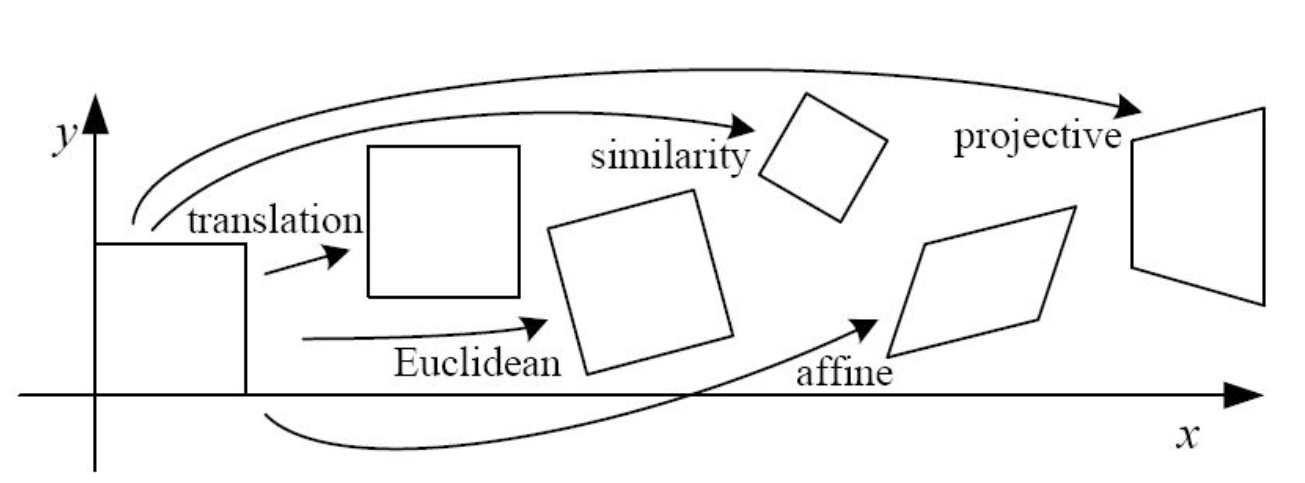
\includegraphics[width=0.9\linewidth]{images/part2/geometric-transformations.png}
\end{figure}

\textbf{Translation (2 DOF.)} Shifts the origin; no rotation or distortion.
$$\mathbf{x}' = \mathbf{x} + \mathbf{t}, \qquad \begin{bmatrix}x'\\y'\\1\end{bmatrix} = \begin{bmatrix}1&0&t_x\\0&1&t_y\\0&0&1\end{bmatrix}\begin{bmatrix}x\\y\\1\end{bmatrix}.$$
\emph{Invariants:} all distances, angles, areas, parallelism, and lengths.\\

\textbf{Euclidean/Rigid (3 DOF.)} Rotation $\theta$ plus translation; preserves the shape of objects.
$$\mathbf{x}' = R\mathbf{x}+\mathbf{t}, \qquad \begin{bmatrix}x'\\y'\\1\end{bmatrix} = \begin{bmatrix}\cos\theta&-\sin\theta&t_x\\\sin\theta&\cos\theta&t_y\\0&0&1\end{bmatrix}\begin{bmatrix}x\\y\\1\end{bmatrix},$$
where $R$ is defined to be the rotation matrix,
$$R=
\begin{bmatrix}
    \cos\theta&-\sin\theta& 0\\
    \sin\theta&\cos\theta& 0\\
    0&0&1
\end{bmatrix},
$$
$R\in SO(2)$ satisfies $RR^T=I$, $\det R=1$. \emph{Invariants:} all distances and angles (congruence).\\

\textbf{Similarity (4 DOF.)} Adds uniform scaling $s>0$ to the Euclidean transform.
$$\begin{bmatrix}x'\\y'\\1\end{bmatrix} = \begin{bmatrix}s\cos\theta&-s\sin\theta&t_x\\s\sin\theta&s\cos\theta&t_y\\0&0&1\end{bmatrix}\begin{bmatrix}x\\y\\1\end{bmatrix}.$$
\emph{Invariants:} angles, ratios of lengths, shape (but not absolute size). SIFT descriptors are designed to be similarity-invariant.\\

\textbf{Affine (6 DOF.)} Any invertible linear map plus translation; the last row is fixed to $[0,0,1]$.
$$\begin{bmatrix}x'\\y'\\1\end{bmatrix} = \begin{bmatrix}a_{11}&a_{12}&t_x\\a_{21}&a_{22}&t_y\\0&0&1\end{bmatrix}\begin{bmatrix}x\\y\\1\end{bmatrix} = \begin{bmatrix}A&\mathbf{t}\\\mathbf{0}^T&1\end{bmatrix}\begin{bmatrix}x\\y\\1\end{bmatrix},$$
where $A\in GL(2)$. An affine map can be decomposed as 
$$A = R(\theta)\,R(-\phi)\,\begin{bmatrix}\lambda_1&0\\0&\lambda_2\end{bmatrix}R(\phi)$$ 
(rotation $\to$ scale $\to$ un-rotate). \emph{Invariants:} parallelism, ratios of areas, ratios of lengths along parallel lines. Requires 3 point correspondences to estimate.\\

\textbf{Projective / Homography (8 DOF.)} The most general linear map on homogeneous coordinates; the last row is free (but $H$ is defined only up to a global scale factor, so $8$ free parameters).
$$\tilde{\mathbf{x}}' = H\tilde{\mathbf{x}}, \quad H = \begin{bmatrix}h_{11}&h_{12}&h_{13}\\h_{21}&h_{22}&h_{23}\\h_{31}&h_{32}&h_{33}\end{bmatrix},$$

$$\mathbf{x}' = \frac{1}{h_{31}x+h_{32}y+h_{33}}\begin{bmatrix}h_{11}x+h_{12}y+h_{13}\\h_{21}x+h_{22}y+h_{23}\end{bmatrix}.$$

\emph{Invariants:} straight lines and cross-ratio of four collinear points. A homography relates any two views of a planar surface (or two views taken from the same camera center). Requires 4 point correspondences to estimate.

\begin{center}
\begin{tabular}{@{}lccl@{}}
\toprule
Transform & DOF & Matrix & Invariants \\
\midrule
Translation  & 2 & $[I\;|\;\mathbf{t}]$ & Distances, angles \\
Euclidean    & 3 & $[R\;|\;\mathbf{t}]$ & Distances, angles \\
Similarity   & 4 & $[sR\;|\;\mathbf{t}]$ & Angles, length ratios \\
Affine       & 6 & $[A\;|\;\mathbf{t}]$ & Parallelism, area ratios \\
Projective   & 8 & $H$ (full $3\times3$) & Lines, cross-ratio \\
\bottomrule
\end{tabular}
\end{center}

% \NoteSection{Homography Estimation - DLT}

% Given $n \ge 4$ point correspondences $\{\mathbf{x}_i \leftrightarrow \mathbf{x}_i'\}$, the \textbf{Direct Linear Transform (DLT)} finds $H$ by forming a linear system. Each correspondence gives two independent equations: stacking all $n$ pairs yields
% $$A\mathbf{h} = \mathbf{0}, \quad A \in \mathbb{R}^{2n\times 9}, \quad \mathbf{h} = \mathrm{vec}(H) \in \mathbb{R}^9.$$
% The solution is the right singular vector of $A$ corresponding to the smallest singular value (via SVD). \textbf{Normalisation} (translate centroid to origin, scale so mean distance is $\sqrt{2}$) is critical before running DLT; unnormalised coordinates cause severe numerical conditioning problems.


\NoteSubsection{How to Determine a 2D Affine Transform}

Suppose we have two triangles $\Delta ABC$ and $\Delta A'B'C'$

\begin{figure}[H]
    \centering
    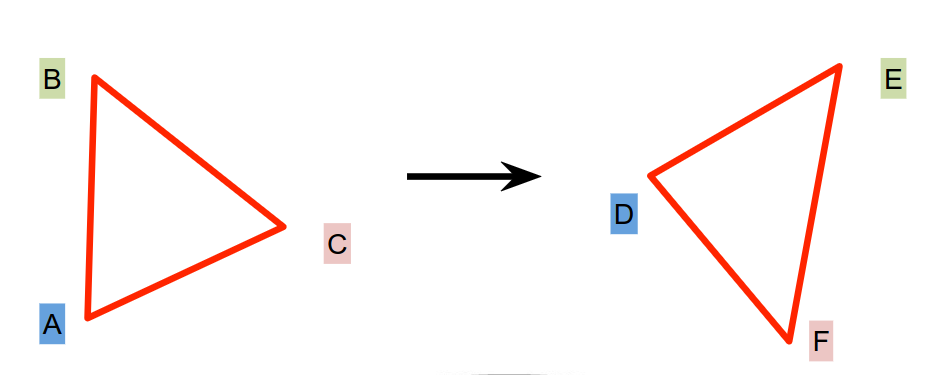
\includegraphics[width=0.5\linewidth]{images/part2/two-triangles.png}
\end{figure}

How do we determine which transformations were applied to $\Delta ABC$ to form $\Delta DEF$? That is, suppose all the points in ABC is $\mathrm{x}$, how do we determine the transformation $M$ such that
$$\mathrm{x}' = M\mathrm{x}$$

\textbf{Setup.} A 2D affine transform in homogeneous coordinates is
$$\begin{bmatrix}x'\\y'\\1\end{bmatrix} = \underbrace{\begin{bmatrix}a & b & t_x \\ c & d & t_y \\ 0 & 0 & 1\end{bmatrix}}_{M}\begin{bmatrix}x\\y\\1\end{bmatrix},$$
giving two scalar equations per correspondence:
$$x' = ax + by + t_x, \qquad y' = cx + dy + t_y.$$
There are 6 unknowns $(a,b,c,d,t_x,t_y)$, so \textbf{3 point correspondences} (6 equations) are necessary and sufficient --- exactly what a triangle provides.\\

\textbf{Linear system.} Stack the correspondences $A\!\to\!D$, $B\!\to\!E$, $C\!\to\!F$ into the system $P\,\mathbf{m} = \mathbf{q}$:
$$
\underbrace{
\begin{bmatrix}
x_A & y_A & 1 & 0   & 0   & 0 \\
0   & 0   & 0 & x_A & y_A & 1 \\
x_B & y_B & 1 & 0   & 0   & 0 \\
0   & 0   & 0 & x_B & y_B & 1 \\
x_C & y_C & 1 & 0   & 0   & 0 \\
0   & 0   & 0 & x_C & y_C & 1
\end{bmatrix}
}_{\mathbf{m}}
\begin{bmatrix}a\\b\\t_x\\c\\d\\t_y\end{bmatrix}
=
\begin{bmatrix}x_A'\\y_A'\\x_B'\\y_B\\x_D'\\y_D'\end{bmatrix}.$$

\textbf{Solution.} Since $P$ is $6\times6$ and non-singular (invertible) (provided the three source points are not collinear), the unique solution is $\mathbf{m} = P^{-1}\mathbf{q}$. Reconstruct $M$ from $\mathbf{m}$ and the fixed last row.

\emph{Note:} if the source points are collinear, $P$ is singular and the affine transform is underdetermined --- the triangle degenerates and no unique map exists.\\

\textbf{More than 3 points: exact vs.\ noisy.} With $n > 3$ correspondences, the system $P\mathbf{m} = \mathbf{q}$ is overdetermined ($P \in \mathbb{R}^{2n\times6}$). Two cases arise:

\begin{itemize}
  \item \emph{Noise-free data.} If all $n$ correspondences are exactly consistent with a single affine map (e.g.\ the corners of a square mapped to a parallelogram), then any 3 non-collinear points already determine $M$ uniquely, and every additional point is automatically satisfied --- the extra rows of $P$ are redundant. You can simply pick 3 points and solve the $6\times6$ system.
  \item \emph{Noisy data.} Real measurements have noise, so no single $M$ satisfies all equations simultaneously. The system is inconsistent and the best we can do is minimize the sum of squared residuals:
  $$\min_{\mathbf{m}}\;\|P\mathbf{m} - \mathbf{q}\|^2.$$
  The solution is given by the \textbf{normal equations}:
  $$P^T P\,\mathbf{m} = P^T\mathbf{q} \;\implies\; \mathbf{m} = (P^TP)^{-1}P^T\mathbf{q} = P^+\mathbf{q},$$
  where $P^+ = (P^TP)^{-1}P^T$ is the Moore--Penrose pseudoinverse. In practice, solve via QR decomposition or Singular Value Decomposition (SVD) rather than forming $P^TP$ explicitly.
\end{itemize}

The residual $\|P\mathbf{m}^* - \mathbf{q}\|$ measures how well an affine model fits the data; a large residual suggests the true transform is not affine (e.g.\ perspective distortion is present).



\NoteSection{3D Rotations}

\textbf{Rotation group $SO(3)$.} A 3D rotation is a $3\times3$ matrix $R$ satisfying $R^TR=I$ and $\det R=+1$. It has 3 DOF. Key representations:

\textbf{Rotation matrix.} Most natural for composing rotations ($R_3 = R_2 R_1$) and rotating vectors ($\mathbf{x}' = R\mathbf{x}$), but 9 numbers for 3 DOF - must maintain orthogonality constraints.\\

\textbf{Axis-angle / Rodrigues.} Any rotation is a rotation by angle $\theta$ about unit axis $\hat{\mathbf{n}}$. Let $[\hat{\mathbf{n}}]_\times$ denote the skew-symmetric cross-product matrix. Then:
$$R = I + \sin\theta\,[\hat{\mathbf{n}}]_\times + (1-\cos\theta)\,[\hat{\mathbf{n}}]_\times^2.$$
Compact (3 parameters: $\theta\hat{\mathbf{n}}$); numerically unstable near $\theta=0$ or $\theta=\pi$.\\

\textbf{Unit quaternion.} $q = (q_0, \mathbf{q}) = (\cos(\theta/2),\,\sin(\theta/2)\hat{\mathbf{n}}) \in \mathbb{R}^4$, $\|q\|=1$. Rotating a vector: $\mathbf{x}' = q\otimes(0,\mathbf{x})\otimes q^{-1}$. Composing two rotations: quaternion product $q_2\otimes q_1$. No gimbal lock; smooth interpolation via SLERP. $q$ and $-q$ represent the same rotation (double cover of $SO(3)$).\\

\textbf{3D Rigid Transform (6 DOF).} In homogeneous coordinates:
$$\begin{bmatrix}\mathbf{x}'\\1\end{bmatrix} = \begin{bmatrix}R & \mathbf{t}\\\mathbf{0}^T & 1\end{bmatrix}\begin{bmatrix}\mathbf{x}\\1\end{bmatrix}, \quad R\in SO(3),\;\mathbf{t}\in\mathbb{R}^3.$$
This is an element of $SE(3)$, the special Euclidean group. Composition is again matrix multiplication; inversion is $[R^T\;|\;-R^T\mathbf{t}]$.



\columnbreaknofill


\NoteChapter{Wavelet and Other Transforms}

\NoteSection{Preliminaries}

\NoteSubsection{Inner Products and Series Expansions}

All transforms in this chapter expand a signal $f$ in a set of \textbf{basis functions} $\{\phi_k\}$:
$$f(x) = \sum_k c_k\,\phi_k(x), \qquad c_k = \langle f,\phi_k\rangle = \int f(x)\,\phi_k^*(x)\,dx.$$
For a discrete, length-$N$ signal: 
$$c_k = \sum_{x=0}^{N-1} f(x)\,\phi_k^*(x).$$
The set $\{c_k\}$ is the \textbf{forward transform}; recovering $f$ from $\{c_k\}$ is the \textbf{inverse transform}.

\NoteSubsection{Orthogonality and Completeness}

A basis is \textbf{orthonormal} if $\langle\phi_j,\phi_k\rangle = \delta_{jk}$. This gives:
\begin{itemize}
    \item \emph{Simple inversion}: each $c_k$ is computed by a single inner product — no matrix solve.
    \item \emph{Parseval's theorem}: $\sum_x|f(x)|^2 = \sum_k|c_k|^2$ — energy is preserved.
    \item \emph{Best $K$-term approximation}: truncating to the $K$ largest $|c_k|$ minimises the $\ell^2$ reconstruction error over all choices of $K$ coefficients.
\end{itemize}
A basis is \textbf{complete} if it spans the signal space (i.e.\ any $f$ can be expressed exactly). In 2D the inner product generalises to $\langle f,\phi\rangle = \iint f(x,y)\,\phi^*(x,y)\,dx\,dy$.

\NoteSection{Matrix-Based Transforms}

\NoteSubsection{1D Matrix Form}

For a discrete $N$-point signal $\mathbf{f}=[f(0),\ldots,f(N-1)]^T$, the forward transform is
$$\mathbf{T} = A\,\mathbf{f},$$
where the $N\times N$ \textbf{transform matrix} $A$ has rows $[A]_{k,:} = \phi_k^*$ (conjugate-basis-function rows). For an orthogonal (real) transform $A^{-1}=A^T$, so $\mathbf{f} = A^T\mathbf{T}$; for a unitary (complex) transform $A^{-1}=A^H$.

\NoteSubsection{2D Separable Transforms}

If the 2D basis is separable, $\phi_{uv}(x,y)=\phi_u(x)\,\phi_v(y)$, the transform of an $N\times N$ image $F$ is
$$T = A\,F\,A^T, \qquad F = A^T T A \quad \text{(for orthogonal }A\text{)}.$$
\textbf{Computational saving}: applying $A$ to rows then to columns costs $O(N^3)$, vs.\ $O(N^4)$ for a brute-force 2D inner product. All transforms in this chapter (DFT, DCT, WHT, Haar, Slant) are separable.\\

\textbf{Energy compaction.} A transform is practically useful if $T$ is \textbf{sparse}: most energy concentrates in a few coefficients. Quantising the remainder to zero enables compression with minimal perceptual loss.

\NoteSection{Basis Images}

For a separable transform $T=AFA^T$, each coefficient $T(u,v)$ measures the projection of $F$ onto the 2D \textbf{basis image}
$$b_{uv}(x,y) = a_u(x)\,a_v(y),$$
where $a_u$ and $a_v$ are the $u$-th and $v$-th rows of $A$. The image reconstructs as $F = \sum_{u,v}T(u,v)\,b_{uv}$.

\begin{itemize}
    \item \emph{DFT basis images}: complex exponentials $e^{j2\pi(ux+vy)/N}$; constant amplitude, varying phase.
    \item \emph{DCT basis images}: $\cos\!\bigl[\frac{(2x+1)u\pi}{2N}\bigr]\cos\!\bigl[\frac{(2y+1)v\pi}{2N}\bigr]$; smooth at low $(u,v)$, rapidly oscillating at high $(u,v)$.
    \item \emph{Haar basis images}: piecewise-constant patches at different positions and scales.
    \item \emph{WHT basis images}: $\pm1$ checkerboard patterns with increasing sequency.
\end{itemize}
Visualising basis images is the standard way to interpret what information a transform coefficient encodes.

\NoteSection{Motivation}

The DFT provides a \emph{global} frequency analysis: each coefficient $F(u,v)$ depends on every pixel, and a sharp edge at one location spreads its energy across the entire spectrum. This has two practical consequences:

\begin{itemize}
    \item \textit{No spatial localisation}: $|F(u,v)|$ cannot reveal \emph{where} in the image a particular frequency component originates.
    \item \textit{Stationarity assumed}: the DFT implicitly treats frequency content as spatially uniform — a poor model for natural images, which are non-stationary (sky vs.\ face vs.\ text).
\end{itemize}

\textbf{Wavelets} resolve both issues by providing \emph{joint space-frequency} localisation: each wavelet coefficient captures a specific frequency band at a specific spatial location. This makes wavelets the preferred transform for image compression (JPEG 2000), denoising, and multi-scale feature extraction.

\NoteSection{Basis Functions in the Time-Frequency Plane}

A central question in transform design is the \textbf{joint localisation} of basis functions in both the space (time) domain and the frequency domain. The spread of a function $\phi$ in the two domains obeys Heisenberg's uncertainty principle:
$$\Delta x \cdot \Delta\xi \;\geq\; \frac{1}{4\pi},$$
where $\Delta x$ is the RMS spatial width of $|\phi|^2$ and $\Delta\xi$ is its RMS bandwidth. No basis function can be perfectly localised in both domains simultaneously; every transform design is a trade-off.

\NoteSubsection{Short-Time Fourier Transform (STFT)}

The STFT localises analysis by multiplying the signal with a fixed window $g(x-b)$ before computing the Fourier transform:
$$\mathrm{STFT}\{f\}(b,\xi) = \int f(x)\,g^*(x-b)\,e^{-j2\pi\xi x}\,dx.$$
Every tile in the \textbf{time-frequency plane} has the same area $\Delta x \cdot \Delta\xi$ determined by the window. This gives \emph{uniform resolution}: identical time and frequency resolution at all scales. If a short window is chosen for good time resolution, frequency resolution suffers at all frequencies — there is no way to adapt.

\NoteSubsection{Wavelet Time-Frequency Tiling}

The CWT replaces the fixed window with a scaled-and-shifted wavelet $\psi_{a,b}(x)=|a|^{-1/2}\psi\!\bigl(\frac{x-b}{a}\bigr)$. Scaling changes the tile shape while preserving its area:
\begin{itemize}
    \item \emph{Small $a$ (high frequency)}: compressed wavelet $\to$ narrow spatial window, wide frequency band — good \textbf{time} resolution.
    \item \emph{Large $a$ (low frequency)}: stretched wavelet $\to$ wide spatial window, narrow frequency band — good \textbf{frequency} resolution.
\end{itemize}
This \textbf{dyadic tiling} matches natural image statistics: transients (edges) are narrow in space and appear at high frequencies; smooth regions are broad and contain mainly low frequencies. The DWT discretises this tiling at octave-band scales.

\begin{center}
\begin{tabular}{@{}lccl@{}}
\toprule
Transform & Space local. & Frequency local. & Tiling \\
\midrule
DFT  & None & Perfect & N/A (global) \\
STFT & Fixed window & Fixed band & Uniform rectangles \\
CWT  & $\propto a$ & $\propto 1/a$ & Dyadic (octave-band) \\
DWT  & Dyadic grid & Octave-band & Dyadic \\
\bottomrule
\end{tabular}
\end{center}

\NoteSection{Continuous Wavelet Transform (CWT)}

The \textbf{CWT} of a 1D signal $f(x)$ is
$$W(a, b) = \frac{1}{\sqrt{|a|}} \int_{-\infty}^{\infty} f(x)\, \psi^*\!\left(\frac{x-b}{a}\right) dx,$$
where
\begin{itemize}
    \item $\psi(x)$ is the \textbf{mother wavelet} --- a zero-mean, unit-energy oscillating function.
    \item $a > 0$ is the \textbf{scale}: large $a$ $\to$ stretched wavelet $\to$ low frequency; small $a$ $\to$ compressed wavelet $\to$ high frequency.
    \item $b$ is the \textbf{translation} (spatial location).
    \item $1/\sqrt{|a|}$ normalises so every scaled copy has unit $L^2$ norm.
\end{itemize}

\textbf{Admissibility condition.} For the inverse to exist, $\psi$ must satisfy
$$C_\psi = \int_0^{\infty} \frac{|\Psi(\omega)|^2}{\omega}\,d\omega < \infty,$$
where $\Psi$ is the Fourier transform of $\psi$. This forces $\Psi(0) = 0$, i.e.\ $\int \psi(x)\,dx = 0$ (zero mean — the wavelet must be oscillatory, not a smooth bump).

\textbf{Inverse CWT.}
$$f(x) = \frac{1}{C_\psi}\int_0^{\infty}\int_{-\infty}^{\infty} W(a,b)\,\frac{1}{\sqrt{a}}\psi\!\left(\frac{x-b}{a}\right)\frac{db\,da}{a^2}.$$

The CWT is continuously parameterised and highly redundant; the DWT discretises it efficiently.

\NoteSection{Multiresolution Analysis (MRA)}

MRA (Mallat, 1989) is the algebraic foundation that converts the CWT into a fast discrete algorithm. An MRA is a nested sequence of subspaces of $L^2(\mathbb{R})$:
$$\cdots \subset V_2 \subset V_1 \subset V_0 \subset V_{-1} \subset \cdots$$
with $\bigcup_j V_j$ dense and $\bigcap_j V_j = \{0\}$. The key axiom is that $f(x)\in V_j$ if and only if $f(2x)\in V_{j-1}$ (halving scale moves up one level), and a \textbf{scaling function} $\phi\in V_0$ generates an orthonormal basis $\{\phi(x-n)\}_{n\in\mathbb{Z}}$ for $V_0$.\\

\textbf{Detail (wavelet) spaces.} The complement $W_j = V_{j-1}\ominus V_j$ captures the detail lost when moving from $V_{j-1}$ to $V_j$. A \textbf{mother wavelet} $\psi$ generates an orthonormal basis for $W_j$:
$$\{2^{-j/2}\psi(2^{-j}x - n) : n\in\mathbb{Z}\}.$$
The decomposition $V_0 = W_1\oplus W_2\oplus\cdots\oplus V_J$ is the multi-level wavelet expansion.\\

\textbf{Two-scale equations.} Both $\phi$ and $\psi$ satisfy refinement relations:
\begin{align*}
\phi(x) &= \sqrt{2}\sum_n h_0[n]\,\phi(2x-n), \\
\psi(x) &= \sqrt{2}\sum_n h_1[n]\,\phi(2x-n),
\end{align*}
where $h_0$ is the \textbf{low-pass (scaling) filter} and $h_1$ is the \textbf{high-pass (wavelet) filter}. These two sequences completely characterise the wavelet basis.

\NoteSection{Discrete Wavelet Transform (DWT)}

\NoteSubsection{1D DWT via Filter Banks}

The DWT samples the CWT at dyadic scales $a=2^j$. By the MRA, one level of decomposition is equivalent to convolving with $h_0$ and $h_1$ and downsampling by 2:
\begin{align*}
a_j[n] &= \sum_k h_0[k-2n]\,a_{j-1}[k] \quad \text{(approximation / low-pass)}\\
d_j[n] &= \sum_k h_1[k-2n]\,a_{j-1}[k] \quad \text{(detail / high-pass)}
\end{align*}
Starting from $a_0 = f$, apply this recursively to $a_j$ for $j=1,\ldots,J$. The full decomposition is:
$$\underbrace{a_J}_{\text{coarse approx}} \;\oplus\; d_J \;\oplus\; d_{J-1} \;\oplus\; \cdots \;\oplus\; d_1.$$

\textbf{Reconstruction (inverse DWT).} Upsample by 2 (insert zeros), then convolve with synthesis filters and sum:
$$a_{j-1}[n] = \sum_k a_j[k]\,\tilde{h}_0[n-2k] + \sum_k d_j[k]\,\tilde{h}_1[n-2k].$$
For orthogonal wavelets $\tilde{h}_0 = h_0$ and $\tilde{h}_1 = h_1$; for biorthogonal wavelets they differ.\\

\textbf{Complexity.} Each level processes a signal half as long as the previous: total work $N + N/2 + N/4 + \cdots = 2N \Rightarrow O(N)$. Compare $O(N\log N)$ for the FFT. No redundancy: total coefficients $= N$.

\NoteSubsection{Haar Wavelet}

The simplest orthonormal wavelet:
$$\phi(x) = \mathbf{1}_{[0,1)}(x), \qquad \psi(x) = \begin{cases}+1, & 0\le x < \tfrac{1}{2},\\ -1, & \tfrac{1}{2}\le x < 1,\\ 0, & \text{otherwise.}\end{cases}$$
Filter coefficients:
$$h_0 = \tfrac{1}{\sqrt{2}}\begin{bmatrix}1&1\end{bmatrix}, \qquad h_1 = \tfrac{1}{\sqrt{2}}\begin{bmatrix}1&-1\end{bmatrix}.$$
One level of the Haar DWT on $(s_0,s_1,s_2,s_3)$ produces:
\begin{itemize}
    \item Approximation: $\frac{s_0+s_1}{\sqrt{2}},\,\frac{s_2+s_3}{\sqrt{2}}$ (pairwise averages)
    \item Detail: $\frac{s_0-s_1}{\sqrt{2}},\,\frac{s_2-s_3}{\sqrt{2}}$ (pairwise differences)
\end{itemize}
The Haar wavelet has only 1 vanishing moment, discontinuous $\psi$, and poor frequency selectivity — it produces visible step artefacts in images. It is used where simplicity and integer arithmetic are paramount (lossless coding, teaching).

\NoteSubsection{Vanishing Moments and Wavelet Families}

A wavelet $\psi$ has $p$ \textbf{vanishing moments} if $\int x^k\psi(x)\,dx = 0$ for $k=0,1,\ldots,p-1$. Vanishing moments cause $d_j[n]$ to be \emph{exactly zero} wherever the signal is a polynomial of degree $\le p-1$, producing sparse coefficient vectors and better compression.

\begin{itemize}
    \item \textbf{Daubechies (dbN).} Maximum vanishing moments ($p=N$) for the shortest orthogonal filter (length $2N$). db1 = Haar. db4 has 4 vanishing moments, 8-tap filters, and smooth appearance. Higher $N$ $\to$ better frequency selectivity but larger spatial support. Asymmetric.

    \item \textbf{Biorthogonal (e.g., 9/7 and 5/3).} Use separate analysis/synthesis filters, allowing \emph{symmetric} (linear-phase) filters — critical for avoiding edge distortions. The \textbf{9/7} float wavelet underlies lossy JPEG~2000; the \textbf{5/3} integer wavelet gives lossless JPEG~2000. Not orthogonal ($h_0\neq\tilde h_0$) but perfectly reconstructing.

    \item \textbf{Symmlets (symN).} Modified Daubechies with near-linear phase; visually cleaner than dbN for image processing.

    \item \textbf{Coiflets (coifN).} Both $\phi$ and $\psi$ have $2N$ vanishing moments; nearly symmetric. Useful when coefficients at all scales should be near-zero for smooth signals.
\end{itemize}

\NoteSection{2D DWT for Images}

The 2D DWT is computed \textbf{separably}: apply the 1D DWT to rows, then to columns. At each level this yields four sub-bands:

\begin{center}
\begin{tabular}{@{}lll@{}}
\toprule
Sub-band & Filtering & Content \\
\midrule
LL & Low-pass rows, Low-pass columns & Coarse approximation \\
LH & Low-pass rows, High-pass columns & Horizontal edges \\
HL & High-pass rows, Low-pass columns & Vertical edges \\
HH & High-pass rows, High-pass columns & Diagonal texture \\
\bottomrule
\end{tabular}
\end{center}

The LL sub-band (size $M/2 \times N/2$) is recursively decomposed for $J$ levels, forming the \textbf{wavelet pyramid}. After $J$ levels: one LL sub-band at $M/2^J\times N/2^J$, plus $3J$ detail sub-bands (LH, HL, HH at each level). Total coefficients $= MN$ (no redundancy).\\

\textbf{Example: one-level decomposition of a $512\times512$ image.}
\begin{itemize}
    \item LL: $256\times256$ (coarse image)
    \item LH: $256\times256$ (horizontal edges — responds to horizontal intensity changes)
    \item HL: $256\times256$ (vertical edges)
    \item HH: $256\times256$ (diagonal edges and fine texture)
\end{itemize}

\textbf{Energy compaction.} For a typical photograph, $\sim$90\% of the energy is in the LL sub-band after 1 level; after 3 levels the LL holds $\sim$99\%. Detail coefficients outside edges are near zero — this sparsity drives compression.

\NoteSection{Wavelet Denoising (Shrinkage)}

The transform-domain denoiser promised in DENOISING, now that the machinery it needs is in place.

\textbf{Algorithm} (Donoho \& Johnstone, 1994):
\begin{enumerate}
    \item Compute the DWT of the noisy image $g = f + \eta$.
    \item \textbf{Threshold} all detail coefficients (leave LL unchanged):
    \begin{itemize}
        \item \emph{Hard}: $\hat{d} = d\cdot\mathbf{1}[|d|>\lambda]$. Preserves large coefficients exactly; can leave isolated spikes.
        \item \emph{Soft}: $\hat{d} = \mathrm{sign}(d)\max(|d|-\lambda,0)$. Biases large coefficients toward zero; gives smoother output.
    \end{itemize}
    \item Invert the DWT to recover $\hat{f}$.
\end{enumerate}
\textbf{Universal threshold.} $\lambda = \hat\sigma\sqrt{2\log N}$, where $\hat\sigma = \mathrm{median}(|d_1|)/0.6745$ is estimated from the finest-scale detail sub-band. This minimises worst-case $\ell^2$ risk.\\

\textbf{Why it works.} Natural image structure is \emph{sparse} in the wavelet domain: a few large coefficients capture edges and textures; Gaussian noise is distributed uniformly across all scales. Thresholding kills the noise floor while preserving signal spikes.


\NoteSection{Shift-Invariant Variants}

The standard downsampled DWT is \textbf{not} shift-invariant: shifting the input by one pixel can completely rearrange which coefficients are large. For edge detection and denoising this is undesirable.

\begin{itemize}
    \item \textbf{Undecimated (Stationary) DWT.} Omit the downsampling step; every level produces full-resolution coefficient arrays. Cost: $O(N J)$; redundancy factor: $O(J)$. Fully shift-invariant.
    \item \textbf{Dual-Tree Complex Wavelet Transform (DT-CWT).} Two parallel real DWTs, offset by $\pi/2$ in phase. The complex coefficients $d^{(1)} + jd^{(2)}$ are approximately analytic. Provides 6 oriented sub-bands (vs.\ 3 for the real DWT) at $\pm15^\circ$, $\pm45^\circ$, $\pm75^\circ$. Approximately shift-invariant at $2\times$ redundancy per level.
\end{itemize}

\NoteSection{Walsh–Hadamard Transform (WHT)}

The WHT is a real, orthogonal transform using only $\pm1$ entries — no multiplications, only additions. The $N\times N$ Hadamard matrix ($N=2^n$) is defined recursively:
$$H_0 = [1], \qquad H_n = \frac{1}{\sqrt{2}}\begin{bmatrix}H_{n-1} & H_{n-1}\\H_{n-1} & -H_{n-1}\end{bmatrix}.$$
The WHT of $\mathbf{f}$ is $\mathbf{F} = H_n \mathbf{f}$ and the inverse is $H_n^{-1} = H_n^T$ (i.e.\ $H_n$ is its own inverse up to scaling).\\

\textbf{Sequency ordering.} In the Walsh ordering, rows of $H_n$ are arranged by the number of sign changes (\emph{sequency}), the square-wave analogue of frequency. Low sequency $\to$ slow variation; high sequency $\to$ rapid sign changes.\\

\textbf{Computation.} Like the FFT, the WHT has a radix-2 butterfly structure and costs $O(N\log N)$ additions — no multiplications at all. This makes it attractive for hardware-constrained applications.\\

\textbf{Applications.}
\begin{itemize}
    \item VP8/WebP: the WHT decorrelates the sixteen $4\times4$ luma DC values within each macroblock before quantisation.
    \item Compressed sensing: random $\pm1$ measurement matrices are Hadamard-based.
    \item Optical multiplexing (Hadamard spectroscopy): measuring $N$ wavelength channels simultaneously with $\log_2 N$ detectors via binary masks.
    \item Fast texture descriptors in resource-limited embedded vision.
\end{itemize}

\NoteSection{Karhunen–Loève Transform (KLT / PCA)}

The KLT is the \textbf{statistically optimal} linear transform for a given signal class. It finds the orthonormal basis that maximises the variance captured by the first $K$ coefficients.\\

\textbf{Computation.}
\begin{enumerate}
    \item Extract $n$ image patches $\{f_i\}\subset\mathbb{R}^N$; compute the mean $\bar{f} = \frac{1}{n}\sum_i f_i$.
    \item Form the $N\times N$ covariance matrix $\Sigma = \frac{1}{n}\sum_i (f_i-\bar{f})(f_i-\bar{f})^T$.
    \item Compute the eigendecomposition $\Sigma = U\Lambda U^T$ (columns of $U$ sorted by descending eigenvalue $\lambda_k$).
    \item The KLT coefficient vector is $\mathbf{c} = U^T(f - \bar{f})$.
\end{enumerate}

\textbf{Optimality.} For a fixed number $K$ of retained coefficients, the KLT minimises the mean-squared reconstruction error among all orthonormal transforms:
$$\hat{f} = \bar{f} + \sum_{k=1}^K c_k\,u_k, \qquad \text{MSE} = \sum_{k=K+1}^N \lambda_k.$$

\textbf{Key properties.}
\begin{itemize}
    \item \emph{Decorrelation}: $\mathrm{Cov}(\mathbf{c}) = \Lambda$ (diagonal) — coefficients are uncorrelated.
    \item \emph{Energy compaction}: the first $K$ eigenvectors capture the maximum possible variance.
    \item \emph{Data-dependent}: the basis $U$ must be recomputed for each dataset; unlike the DCT or DFT it has no fast algorithm.
    \item \emph{Complexity}: the covariance matrix is $N\times N$ — feasible for small patches ($16\times16$, $N=256$) but not for full images. The dual-space trick (SVD of the $N\times n$ data matrix) reduces cost to $O(n^2)$ when $n \ll N$.
\end{itemize}

\textbf{Relation to DCT.} For first-order Markov (AR(1)) signals with high inter-pixel correlation $\rho\to1$, the KLT eigenvectors converge to DCT basis functions. This explains why the DCT is a near-optimal transform for typical image blocks.\\

\textbf{Applications.}
\begin{itemize}
    \item \emph{Eigenfaces} (Turk \& Pentland, 1991): KLT on a face image dataset; each eigenvector is an "eigenface". A new face is represented as a $K$-vector of KLT coefficients and recognised by nearest-neighbour in that subspace.
    \item \emph{Hyperspectral image analysis}: PCA reduces hundreds of spectral channels to a few principal components that capture the dominant material variation.
    \item \emph{Image compression}: patch-level KLT achieves the minimum distortion for a given bit-rate, but its data dependence makes it impractical in general-purpose codecs.
\end{itemize}

\begin{center}
\begin{tabular}{@{}lcccc@{}}
\toprule
Transform & Basis & Shift-inv. & Data-dep. & Cost \\
\midrule
DFT  & Sinusoids & Yes & No & $O(N\log N)$ \\
DCT  & Cosines   & Yes & No & $O(N\log N)$ \\
DWT  & Wavelets  & No  & No & $O(N)$ \\
WHT  & $\pm1$ sq.\ waves & Yes & No & $O(N\log N)$ \\
KLT  & Eigenvectors & Yes & \textbf{Yes} & $O(N^2)$--$O(N^3)$ \\
\bottomrule
\end{tabular}
\end{center}




\end{notes}
\end{document}
